\documentclass[final,a4paper,10pt,abstracton]{scrreprt}

\usepackage{verbatim}

%
% General
\usepackage[english]{babel}
\usepackage{hyperref}
\hypersetup{final,plainpages=false,pagebackref,colorlinks=true,linkcolor=blue,urlcolor=red,citecolor=blue,pdfpagemode=UseOutlines,pdfstartview=FitH,pdfborder={0 0 0}}

\providecommand{\indexed}[1]{\index{#1}#1}

\newcommand{\HRule}{\rule{\linewidth}{0.5mm}}
\newcommand{\ie}{i.\,e.\ }
\newcommand{\eg}{e.\,g.\ }

%
% Graphics
\usepackage{pgfpages}
\usepackage{tikz}
\usetikzlibrary{arrows,positioning,shapes,topaths,calc,fit,backgrounds,matrix,shadows,automata}
\usepackage{soul}

%\usetikzlibrary{intersections}
%\usetikzlibrary{calc}
%\usetikzlibrary{positioning}


%
% Snippets 
\usepackage{moreverb}
\usepackage{listings}

% Tables
%-------------
\usepackage{tabularx}



\title{CernVM Release Testing Walkthrough - Developer Manual}
% \subtitle{Technical Report}
\author{GNU USER}

\providecommand{\cernvmreleasetesting}{{\scshape CernVM Release Testing~}}
\providecommand{\releasetesting}{{\scshape Release Testing~}}
\providecommand{\cern}{{\scshape cern~}}
\providecommand{\cernvm}{{\scshape CernVM~}}
\providecommand{\tapper}{{\scshape Tapper~}}
\providecommand{\amdtapper}{{\scshape AMD Tapper~}}

\providecommand{\todo}[1]{\textcolor{red}{#1}}
\definecolor {light-blue}{rgb}{230,244,255}


\usepackage[nottoc]{tocbibind}

\usepackage{makeidx}
\makeindex

\setcounter{secnumdepth}{4}
\setcounter{tocdepth}{4}

\begin{document}
\selectlanguage{english}
\renewcommand\today{June 2011}

\pagestyle{empty}
\begin{titlepage}
	\begin{addmargin}[-\oddsidemargin]{-\evensidemargin}
  		\newlength{\saveparindent}
		\setlength{\saveparindent}{\parindent}
		\setlength{\parindent}{0cm}

  		\sf
		\center
		\vspace*{-1cm}
		\mbox{
	  		\parbox{4cm}{
				\resizebox{4cm}{!}{\begin{pgfpicture}
\pgfpathmoveto{\pgfqpoint{5.858cm}{9.523cm}}
\pgfpathlineto{\pgfqpoint{16.845cm}{9.523cm}}
\pgfpathlineto{\pgfqpoint{16.845cm}{20.265cm}}
\pgfpathlineto{\pgfqpoint{5.858cm}{20.265cm}}
\pgfpathclose
\pgfusepath{clip}
\begin{pgfscope}
\begin{pgfscope}
\end{pgfscope}
\begin{pgfscope}
\pgfpathmoveto{\pgfqpoint{0cm}{0cm}}
\pgfpathlineto{\pgfqpoint{21cm}{0cm}}
\pgfpathlineto{\pgfqpoint{21cm}{29.7cm}}
\pgfpathlineto{\pgfqpoint{0cm}{29.7cm}}
\pgfpathclose
\pgfusepath{clip}
\definecolor{eps2pgf_color}{rgb}{0.121569,0.337255,0.984314}\pgfsetstrokecolor{eps2pgf_color}\pgfsetfillcolor{eps2pgf_color}
\pgfpathmoveto{\pgfqpoint{8.912cm}{15.808cm}}
\pgfpathcurveto{\pgfqpoint{8.761cm}{15.793cm}}{\pgfqpoint{8.49cm}{15.793cm}}{\pgfqpoint{8.339cm}{15.793cm}}
\pgfpathlineto{\pgfqpoint{8.339cm}{16.471cm}}
\pgfpathlineto{\pgfqpoint{8.851cm}{16.471cm}}
\pgfpathcurveto{\pgfqpoint{8.927cm}{16.471cm}}{\pgfqpoint{9.002cm}{16.456cm}}{\pgfqpoint{9.078cm}{16.456cm}}
\pgfpathcurveto{\pgfqpoint{9.078cm}{16.471cm}}{\pgfqpoint{9.063cm}{16.502cm}}{\pgfqpoint{9.063cm}{16.517cm}}
\pgfpathcurveto{\pgfqpoint{9.063cm}{16.532cm}}{\pgfqpoint{9.078cm}{16.562cm}}{\pgfqpoint{9.078cm}{16.577cm}}
\pgfpathcurveto{\pgfqpoint{9.002cm}{16.577cm}}{\pgfqpoint{8.927cm}{16.562cm}}{\pgfqpoint{8.851cm}{16.562cm}}
\pgfpathlineto{\pgfqpoint{8.339cm}{16.562cm}}
\pgfpathlineto{\pgfqpoint{8.339cm}{17.15cm}}
\pgfpathlineto{\pgfqpoint{8.655cm}{17.15cm}}
\pgfpathlineto{\pgfqpoint{8.912cm}{17.135cm}}
\pgfpathcurveto{\pgfqpoint{8.987cm}{17.135cm}}{\pgfqpoint{9.063cm}{17.12cm}}{\pgfqpoint{9.138cm}{17.12cm}}
\pgfpathcurveto{\pgfqpoint{9.138cm}{17.135cm}}{\pgfqpoint{9.123cm}{17.165cm}}{\pgfqpoint{9.123cm}{17.18cm}}
\pgfpathcurveto{\pgfqpoint{9.123cm}{17.21cm}}{\pgfqpoint{9.138cm}{17.226cm}}{\pgfqpoint{9.138cm}{17.256cm}}
\pgfpathlineto{\pgfqpoint{8.113cm}{17.256cm}}
\pgfpathlineto{\pgfqpoint{8.113cm}{15.687cm}}
\pgfpathlineto{\pgfqpoint{9.153cm}{15.687cm}}
\pgfpathcurveto{\pgfqpoint{9.153cm}{15.702cm}}{\pgfqpoint{9.138cm}{15.732cm}}{\pgfqpoint{9.138cm}{15.748cm}}
\pgfpathcurveto{\pgfqpoint{9.138cm}{15.778cm}}{\pgfqpoint{9.153cm}{15.793cm}}{\pgfqpoint{9.153cm}{15.823cm}}
\pgfpathcurveto{\pgfqpoint{9.078cm}{15.808cm}}{\pgfqpoint{8.987cm}{15.808cm}}{\pgfqpoint{8.912cm}{15.808cm}}
\pgfpathmoveto{\pgfqpoint{11.023cm}{17.256cm}}
\pgfpathlineto{\pgfqpoint{10.933cm}{17.256cm}}
\pgfpathlineto{\pgfqpoint{10.933cm}{15.672cm}}
\pgfpathcurveto{\pgfqpoint{10.948cm}{15.687cm}}{\pgfqpoint{10.978cm}{15.687cm}}{\pgfqpoint{11.008cm}{15.687cm}}
\pgfpathcurveto{\pgfqpoint{11.023cm}{15.687cm}}{\pgfqpoint{11.053cm}{15.687cm}}{\pgfqpoint{11.068cm}{15.672cm}}
\pgfpathlineto{\pgfqpoint{11.068cm}{16.924cm}}
\pgfpathlineto{\pgfqpoint{11.099cm}{16.924cm}}
\pgfpathlineto{\pgfqpoint{12.199cm}{15.823cm}}
\pgfpathcurveto{\pgfqpoint{12.26cm}{15.763cm}}{\pgfqpoint{12.305cm}{15.717cm}}{\pgfqpoint{12.335cm}{15.672cm}}
\pgfpathlineto{\pgfqpoint{12.411cm}{15.672cm}}
\pgfpathlineto{\pgfqpoint{12.411cm}{17.256cm}}
\pgfpathcurveto{\pgfqpoint{12.38cm}{17.256cm}}{\pgfqpoint{12.365cm}{17.241cm}}{\pgfqpoint{12.335cm}{17.241cm}}
\pgfpathcurveto{\pgfqpoint{12.305cm}{17.241cm}}{\pgfqpoint{12.29cm}{17.256cm}}{\pgfqpoint{12.26cm}{17.256cm}}
\pgfpathlineto{\pgfqpoint{12.26cm}{16.064cm}}
\pgfpathlineto{\pgfqpoint{12.245cm}{16.064cm}}
\pgfpathclose
\pgfpathmoveto{\pgfqpoint{7.871cm}{15.928cm}}
\pgfpathcurveto{\pgfqpoint{7.826cm}{15.883cm}}{\pgfqpoint{7.615cm}{15.748cm}}{\pgfqpoint{7.328cm}{15.748cm}}
\pgfpathcurveto{\pgfqpoint{6.936cm}{15.748cm}}{\pgfqpoint{6.65cm}{16.019cm}}{\pgfqpoint{6.65cm}{16.471cm}}
\pgfpathcurveto{\pgfqpoint{6.65cm}{16.848cm}}{\pgfqpoint{6.876cm}{17.195cm}}{\pgfqpoint{7.343cm}{17.195cm}}
\pgfpathcurveto{\pgfqpoint{7.615cm}{17.195cm}}{\pgfqpoint{7.796cm}{17.045cm}}{\pgfqpoint{7.841cm}{16.999cm}}
\pgfpathlineto{\pgfqpoint{7.856cm}{16.999cm}}
\pgfpathcurveto{\pgfqpoint{7.871cm}{17.06cm}}{\pgfqpoint{7.886cm}{17.12cm}}{\pgfqpoint{7.901cm}{17.18cm}}
\pgfpathcurveto{\pgfqpoint{7.735cm}{17.241cm}}{\pgfqpoint{7.539cm}{17.286cm}}{\pgfqpoint{7.358cm}{17.286cm}}
\pgfpathcurveto{\pgfqpoint{6.815cm}{17.286cm}}{\pgfqpoint{6.393cm}{16.984cm}}{\pgfqpoint{6.393cm}{16.471cm}}
\pgfpathcurveto{\pgfqpoint{6.393cm}{15.974cm}}{\pgfqpoint{6.74cm}{15.657cm}}{\pgfqpoint{7.298cm}{15.657cm}}
\pgfpathcurveto{\pgfqpoint{7.494cm}{15.657cm}}{\pgfqpoint{7.705cm}{15.687cm}}{\pgfqpoint{7.856cm}{15.778cm}}
\pgfpathclose
\pgfpathmoveto{\pgfqpoint{9.605cm}{16.532cm}}
\pgfpathlineto{\pgfqpoint{9.605cm}{17.165cm}}
\pgfpathcurveto{\pgfqpoint{9.711cm}{17.165cm}}{\pgfqpoint{9.998cm}{17.18cm}}{\pgfqpoint{10.088cm}{17.165cm}}
\pgfpathcurveto{\pgfqpoint{10.284cm}{17.135cm}}{\pgfqpoint{10.375cm}{17.03cm}}{\pgfqpoint{10.375cm}{16.879cm}}
\pgfpathcurveto{\pgfqpoint{10.375cm}{16.698cm}}{\pgfqpoint{10.239cm}{16.577cm}}{\pgfqpoint{10.043cm}{16.547cm}}
\pgfpathcurveto{\pgfqpoint{9.922cm}{16.517cm}}{\pgfqpoint{9.651cm}{16.532cm}}{\pgfqpoint{9.605cm}{16.532cm}}
\pgfpathmoveto{\pgfqpoint{10.616cm}{15.868cm}}
\pgfpathlineto{\pgfqpoint{10.088cm}{16.471cm}}
\pgfpathcurveto{\pgfqpoint{10.344cm}{16.502cm}}{\pgfqpoint{10.616cm}{16.637cm}}{\pgfqpoint{10.616cm}{16.909cm}}
\pgfpathcurveto{\pgfqpoint{10.616cm}{17.135cm}}{\pgfqpoint{10.435cm}{17.256cm}}{\pgfqpoint{10.043cm}{17.256cm}}
\pgfpathlineto{\pgfqpoint{9.394cm}{17.256cm}}
\pgfpathlineto{\pgfqpoint{9.394cm}{15.672cm}}
\pgfpathcurveto{\pgfqpoint{9.44cm}{15.687cm}}{\pgfqpoint{9.47cm}{15.687cm}}{\pgfqpoint{9.515cm}{15.687cm}}
\pgfpathcurveto{\pgfqpoint{9.545cm}{15.687cm}}{\pgfqpoint{9.59cm}{15.687cm}}{\pgfqpoint{9.621cm}{15.672cm}}
\pgfpathlineto{\pgfqpoint{9.621cm}{16.441cm}}
\pgfpathlineto{\pgfqpoint{9.832cm}{16.441cm}}
\pgfpathlineto{\pgfqpoint{10.028cm}{16.23cm}}
\pgfpathlineto{\pgfqpoint{10.329cm}{15.883cm}}
\pgfpathcurveto{\pgfqpoint{10.39cm}{15.808cm}}{\pgfqpoint{10.435cm}{15.748cm}}{\pgfqpoint{10.495cm}{15.672cm}}
\pgfpathcurveto{\pgfqpoint{10.54cm}{15.687cm}}{\pgfqpoint{10.586cm}{15.687cm}}{\pgfqpoint{10.646cm}{15.687cm}}
\pgfpathcurveto{\pgfqpoint{10.691cm}{15.687cm}}{\pgfqpoint{10.736cm}{15.687cm}}{\pgfqpoint{10.782cm}{15.672cm}}
\pgfpathlineto{\pgfqpoint{10.736cm}{15.732cm}}
\pgfpathclose
\pgfpathmoveto{\pgfqpoint{9.163cm}{12.394cm}}
\pgfpathcurveto{\pgfqpoint{8.998cm}{12.418cm}}{\pgfqpoint{8.836cm}{12.452cm}}{\pgfqpoint{8.677cm}{12.496cm}}
\pgfpathcurveto{\pgfqpoint{9.079cm}{12.099cm}}{\pgfqpoint{9.564cm}{11.791cm}}{\pgfqpoint{10.102cm}{11.601cm}}
\pgfpathlineto{\pgfqpoint{10.285cm}{11.802cm}}
\pgfpathcurveto{\pgfqpoint{9.877cm}{11.933cm}}{\pgfqpoint{9.497cm}{12.134cm}}{\pgfqpoint{9.163cm}{12.394cm}}
\pgfpathmoveto{\pgfqpoint{8.327cm}{17.627cm}}
\pgfpathlineto{\pgfqpoint{8.641cm}{17.624cm}}
\pgfpathcurveto{\pgfqpoint{9.035cm}{18.135cm}}{\pgfqpoint{10.046cm}{18.893cm}}{\pgfqpoint{11.403cm}{18.893cm}}
\pgfpathcurveto{\pgfqpoint{11.698cm}{18.893cm}}{\pgfqpoint{11.985cm}{18.857cm}}{\pgfqpoint{12.259cm}{18.79cm}}
\pgfpathcurveto{\pgfqpoint{12.152cm}{18.903cm}}{\pgfqpoint{12.036cm}{19.008cm}}{\pgfqpoint{11.914cm}{19.106cm}}
\pgfpathcurveto{\pgfqpoint{11.747cm}{19.128cm}}{\pgfqpoint{11.576cm}{19.141cm}}{\pgfqpoint{11.403cm}{19.141cm}}
\pgfpathcurveto{\pgfqpoint{10.19cm}{19.141cm}}{\pgfqpoint{9.068cm}{18.589cm}}{\pgfqpoint{8.327cm}{17.627cm}}
\pgfpathmoveto{\pgfqpoint{11.403cm}{11.624cm}}
\pgfpathcurveto{\pgfqpoint{11.229cm}{11.624cm}}{\pgfqpoint{11.059cm}{11.639cm}}{\pgfqpoint{10.891cm}{11.663cm}}
\pgfpathlineto{\pgfqpoint{10.691cm}{11.444cm}}
\pgfpathcurveto{\pgfqpoint{10.923cm}{11.401cm}}{\pgfqpoint{11.161cm}{11.377cm}}{\pgfqpoint{11.403cm}{11.377cm}}
\pgfpathcurveto{\pgfqpoint{12.506cm}{11.377cm}}{\pgfqpoint{13.503cm}{11.84cm}}{\pgfqpoint{14.21cm}{12.581cm}}
\pgfpathlineto{\pgfqpoint{14.142cm}{12.873cm}}
\pgfpathcurveto{\pgfqpoint{13.475cm}{12.109cm}}{\pgfqpoint{12.495cm}{11.624cm}}{\pgfqpoint{11.403cm}{11.624cm}}
\pgfpathmoveto{\pgfqpoint{14.64cm}{13.119cm}}
\pgfpathcurveto{\pgfqpoint{14.956cm}{13.596cm}}{\pgfqpoint{15.169cm}{14.147cm}}{\pgfqpoint{15.248cm}{14.738cm}}
\pgfpathlineto{\pgfqpoint{15.265cm}{14.736cm}}
\pgfpathlineto{\pgfqpoint{15.889cm}{19.191cm}}
\pgfpathlineto{\pgfqpoint{15.643cm}{19.226cm}}
\pgfpathlineto{\pgfqpoint{15.2cm}{16.058cm}}
\pgfpathcurveto{\pgfqpoint{14.939cm}{17.301cm}}{\pgfqpoint{14.082cm}{18.327cm}}{\pgfqpoint{12.942cm}{18.822cm}}
\pgfpathcurveto{\pgfqpoint{13.044cm}{18.688cm}}{\pgfqpoint{13.138cm}{18.548cm}}{\pgfqpoint{13.223cm}{18.403cm}}
\pgfpathcurveto{\pgfqpoint{14.307cm}{17.773cm}}{\pgfqpoint{15.038cm}{16.6cm}}{\pgfqpoint{15.038cm}{15.259cm}}
\pgfpathcurveto{\pgfqpoint{15.038cm}{14.605cm}}{\pgfqpoint{14.863cm}{13.992cm}}{\pgfqpoint{14.56cm}{13.462cm}}
\pgfpathclose
\pgfpathmoveto{\pgfqpoint{7.769cm}{15.259cm}}
\pgfpathlineto{\pgfqpoint{7.77cm}{15.344cm}}
\pgfpathlineto{\pgfqpoint{7.522cm}{15.35cm}}
\pgfpathlineto{\pgfqpoint{7.521cm}{15.259cm}}
\pgfpathcurveto{\pgfqpoint{7.521cm}{14.938cm}}{\pgfqpoint{7.56cm}{14.619cm}}{\pgfqpoint{7.638cm}{14.31cm}}
\pgfpathcurveto{\pgfqpoint{7.724cm}{13.965cm}}{\pgfqpoint{7.857cm}{13.642cm}}{\pgfqpoint{8.026cm}{13.344cm}}
\pgfpathcurveto{\pgfqpoint{8.161cm}{13.268cm}}{\pgfqpoint{8.303cm}{13.202cm}}{\pgfqpoint{8.448cm}{13.143cm}}
\pgfpathcurveto{\pgfqpoint{8.189cm}{13.506cm}}{\pgfqpoint{7.992cm}{13.918cm}}{\pgfqpoint{7.878cm}{14.371cm}}
\pgfpathcurveto{\pgfqpoint{7.805cm}{14.659cm}}{\pgfqpoint{7.769cm}{14.958cm}}{\pgfqpoint{7.769cm}{15.259cm}}
\pgfpathmoveto{\pgfqpoint{13.376cm}{16.381cm}}
\pgfpathcurveto{\pgfqpoint{13.376cm}{14.377cm}}{\pgfqpoint{11.745cm}{12.747cm}}{\pgfqpoint{9.741cm}{12.747cm}}
\pgfpathcurveto{\pgfqpoint{8.072cm}{12.747cm}}{\pgfqpoint{6.622cm}{13.876cm}}{\pgfqpoint{6.216cm}{15.493cm}}
\pgfpathcurveto{\pgfqpoint{6.144cm}{15.782cm}}{\pgfqpoint{6.107cm}{16.081cm}}{\pgfqpoint{6.107cm}{16.381cm}}
\pgfpathcurveto{\pgfqpoint{6.107cm}{18.385cm}}{\pgfqpoint{7.737cm}{20.016cm}}{\pgfqpoint{9.741cm}{20.016cm}}
\pgfpathcurveto{\pgfqpoint{11.745cm}{20.016cm}}{\pgfqpoint{13.376cm}{18.385cm}}{\pgfqpoint{13.376cm}{16.381cm}}
\pgfpathmoveto{\pgfqpoint{9.741cm}{20.263cm}}
\pgfpathcurveto{\pgfqpoint{7.601cm}{20.263cm}}{\pgfqpoint{5.859cm}{18.522cm}}{\pgfqpoint{5.859cm}{16.381cm}}
\pgfpathcurveto{\pgfqpoint{5.859cm}{16.06cm}}{\pgfqpoint{5.899cm}{15.741cm}}{\pgfqpoint{5.976cm}{15.433cm}}
\pgfpathcurveto{\pgfqpoint{5.984cm}{15.4cm}}{\pgfqpoint{5.995cm}{15.369cm}}{\pgfqpoint{6.004cm}{15.337cm}}
\pgfpathlineto{\pgfqpoint{6.002cm}{15.336cm}}
\pgfpathlineto{\pgfqpoint{6.975cm}{11.854cm}}
\pgfpathlineto{\pgfqpoint{7.214cm}{11.92cm}}
\pgfpathlineto{\pgfqpoint{6.607cm}{14.092cm}}
\pgfpathcurveto{\pgfqpoint{7.321cm}{13.114cm}}{\pgfqpoint{8.47cm}{12.499cm}}{\pgfqpoint{9.741cm}{12.499cm}}
\pgfpathcurveto{\pgfqpoint{10.379cm}{12.499cm}}{\pgfqpoint{10.98cm}{12.654cm}}{\pgfqpoint{11.511cm}{12.928cm}}
\pgfpathlineto{\pgfqpoint{8.408cm}{9.525cm}}
\pgfpathlineto{\pgfqpoint{8.743cm}{9.525cm}}
\pgfpathlineto{\pgfqpoint{12.61cm}{13.765cm}}
\pgfpathlineto{\pgfqpoint{12.608cm}{13.767cm}}
\pgfpathcurveto{\pgfqpoint{13.132cm}{14.341cm}}{\pgfqpoint{13.486cm}{15.073cm}}{\pgfqpoint{13.59cm}{15.882cm}}
\pgfpathlineto{\pgfqpoint{15.075cm}{9.525cm}}
\pgfpathlineto{\pgfqpoint{15.329cm}{9.525cm}}
\pgfpathlineto{\pgfqpoint{13.521cm}{17.264cm}}
\pgfpathlineto{\pgfqpoint{13.521cm}{17.264cm}}
\pgfpathcurveto{\pgfqpoint{13.224cm}{18.532cm}}{\pgfqpoint{12.305cm}{19.564cm}}{\pgfqpoint{11.104cm}{20.016cm}}
\pgfpathlineto{\pgfqpoint{16.843cm}{20.016cm}}
\pgfpathlineto{\pgfqpoint{16.843cm}{20.263cm}}
\pgfusepath{fill}
\end{pgfscope}
\end{pgfscope}
\end{pgfpicture}}
%				
%				%\begin{tikzpicture}[scale=0.5]
%				%	\path[fill=black, join=round] (1,1)--(2,2)--(2,5)--(5,5)--(6,6)--(1,6)--(1,1)--(2,0)--(5,0)--(7,2)--(7,5)--(6,6)--(6,1)--cycle;
%				%	\clip (6,6)--(5,5)--(5,2)--(2,2)--(1,1)--(6,1)--(6,6)--(5,7)--(2,7)--(0,5)--(0,2)--(1,1)--(1,6)--cycle;
%				%	\shade[inner color=green, outer color=black] (3,4) circle(5.5cm);
%				%\end{tikzpicture}
	  		}
	  		\parbox{9cm}{
	    			%\LARGE CERN\\
	    			%\large PH-SFT%\\[0.5cm]
			}
		}
		\vspace*{2.5cm}
 
  		{\large \scshape CernVM Release Testing Walkthrough}\\[0.5cm]
  		\HRule\\[0.4cm]
		\huge CernVM Release Testing Walkthrough \\Developer Manual\\
		\HRule\\[1.5cm]
		
%        \includegraphics[height=5cm]{marbles}\\[1.5cm]
        
\includegraphics{img/IMG_cernvmlogo}\\[1.5cm] 
		\large GNU USER\\[0.4cm]
		%\today
 
		\large Technical Report\\
		Version: 1.6 \today 
		%	\large ISSN 1432-7864	

  		\setlength{\parindent}{\saveparindent}
	\end{addmargin}
\end{titlepage}
\cleardoublepage
\pagenumbering{roman}



\abstract{
The \cernvmreleasetesting\ project is a testing infrastructure for CernVM images, the usecase for the project is to provide an automated
testing environment, which will install and configure CernVM images, run the set of tests and report the results on a web interface.
}

\tableofcontents
\clearpage
\pagenumbering{arabic}
\pagestyle{headings}

\chapter{Overview}
\label{sct:overview}

CernVM currently supports images for VirtualBox, VMware, Xen, KVM and Microsoft Hyper-V hypervisors, each new release of a CernVM image needs to be 
thoroughly tested on each supported platform and hypervisor. The \cernvmreleasetesting\ project is designed to meet this requirement by providing an 
automated testing environment for CernVM images, which will install and configure CernVM images, run the set of tests and report the results on a web
interface.

The intent of this document is to provided a step-by-step guide on setting up an entire \cernvmreleasetesting\ infrastructure, including instructions
on how to set up and configure test clients, the main server running the web interface and database, as well as writing and executing tests. If you are
new to release testing and want a document to guide you through the entire process of setting up a working \cernvmreleasetesting\ infrastructure,
then this guide for you.

All the code needed to setup the entire \releasetesting\ infrastructure for CernVM image testing, is located at the \cernvmreleasetesting\ Google Code project
page\cite{GCreleasetesting} including this document and all other documentation. 

While this document is not intended to be a replacement for the reference manual, the following is a brief description of the \releasetesting\ infrastructure 
including an introduction to the core component, \amdtapper\cite{tapper}. Figure~\ref{fig:architecture} consists of a diagram outlining the
\indexed{\tapper~Architecture}, which consists of test clients and a server, the server is what controls the test clients, gathers 
results, and then displays the results through a web interface.\newline

\begin{figure}[!hbp]
	\begin{center}
		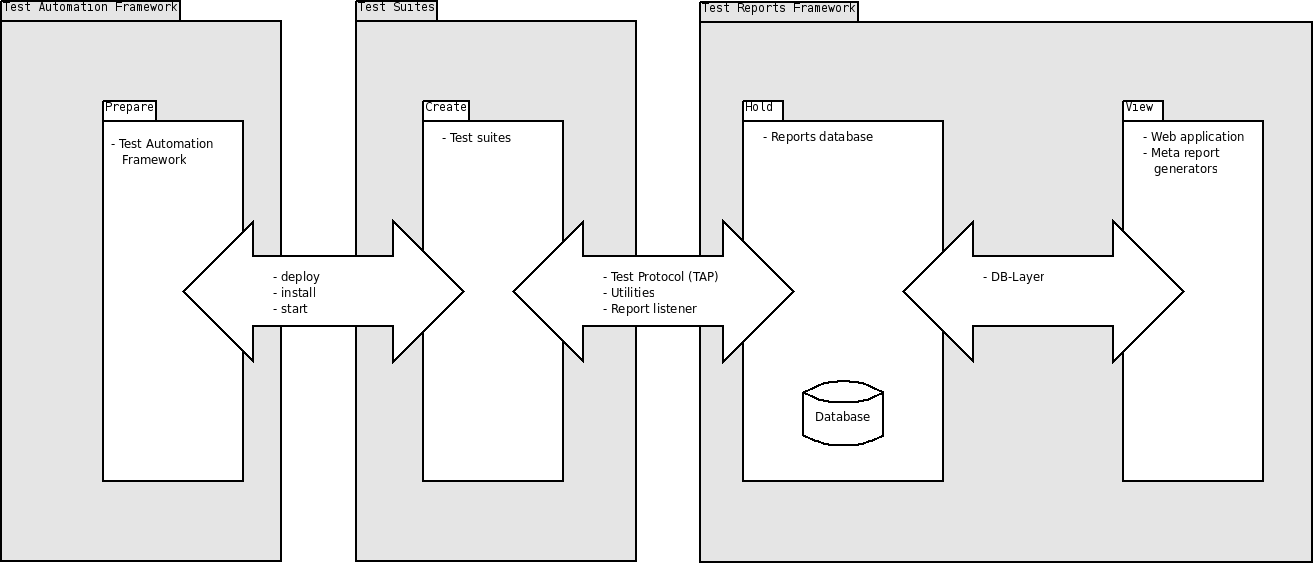
\includegraphics[scale=0.25]{img/tapper_architecture_overview.png}
	\end{center}
	\caption{Overview of the \tapper architecture}
	\label{fig:architecture}
\end{figure}

The components of the \releasetesting~Framework are listed in Table~\ref{tbl:components}. 

\begin{table}
  \begin{center}

    \begin{tabularx}{\linewidth}{l|X}
      {\bf\centering \releasetesting component name} & {\bf\centering Description} \\\hline
%        \texttt{Agent} & Communicates with service insances and requests a job to execute. Upon receiving the job downloads the input 
%                         files, executes the job, uploads job output files and reports that the job execution is finished. \\
%        \texttt{Generic Job and Storage Manager} & Distributes jobs from the internal queue to Agents for execution, provides space for storing 
%                                                   the job output   \\
%        \texttt{AliEn Job Manager} & Retrieves jobs from the central task queue of \indexed{AliEn} Grid \cite{alien} and sends them to 
%                                     Agents for execution \\
%        \texttt{AliEn Storage Manager} & Uploads the output of AliEn jobs executed by Agents and finalizes the job status in AliEn Grid.  \\
%        \texttt{PanDA Storage Manager} & Uploads the output of \indexed{PanDA} \cite{panda} jobs executed by Agents and finalizes the job status in PanDA Grid  \\
    \end{tabularx}  
  \end{center}

  \caption{List of \releasetesting and \amdtapper components}

  \label{tbl:components}
\end{table}

\chapter{\cernvmreleasetesting Test Client Platform Setup}
\label{sec:testclientsetup}

\section{Introduction}
The intent of this document is to provided a step-by-step guide on setting up an entire \cernvmreleasetesting\ infrastructure, including 
instructions on how to set up and configure test clients, the main server running the web interface and database, as well as writing and 
executing tests. If you are new to release testing and want a document to guide you through the entire process of setting up a working
 \cernvmreleasetesting\ infrastructure, then this guide for you.

This section provides complete step by step instructions on how to setup and configure the test clients which are part of a basic working
\releasetesting environment by outlining the procedure for setting up test clients on numerous platforms, hence why this is called a 
\emph{walkthrough} document. This guide is intended for users familiar enough with computers and desktop environments to enter basic commands
in a terminal and install various operating systems. 

As this guide is directed towards users who are new to \cernvmreleasetesting and \tapper and
are interested in quickly getting a \cernvm testing infrastructure quickly set up, many assumptions regarding the requirements necessary are 
made.As is the case, these instructions are provided for a generalized audience based on our own experience and the requirements that we feel 
most users will have, \emph{so feel free to deviate from the instructions}.
\section{Red Hat Based Test Client Setup}
\subsection{Configuring the system}
\label{sec:rhconfig}
\begin{enumerate}
\item 	After the system has booted remove the follow unnecessary startup applications by selecting from the menu  
		\verb|System -> Preferences -> Startup Applications|
\begin{itemize}
\item	bluetooth
\item	evolution alarm
\item	Gnome Login Sound
\item	PackageKit Update Applet
\item	print queue
\item	screensaver
\item	visual assistance/aid
\item	volume control
\item	any others you think are unnecessary based on your own discretion
\end{itemize}

\item	Next enable and configure the remote desktop from the menu \verb|System -> Preferences -> Remote Desktop| and ensure
		that the following options are configured	
\begin{itemize}
\item	Enable the option ``Allow others to view your desktop''
\item	Enable the option ``Allow other users to control your desktop''
\item	Disable the option ``You must confirm access to this machine''
\end{itemize}

\item	Next enable SSH access to the machine, in order for SSH and VNC access to work the firewall will have to be disabled
\begin{itemize}
\item[a.]	First disable the firewall from the menu \verb|System -> Adminisration -> Firewall| and click the ``Disable'' 
			button and then click ``Apply'' to apply the changes! {\bf This is a quick solution for now because it's too 
			much work to configure the firewall for VNC, SSH, Apache, MySQL, PHPMyAdmin, MCP, and all the other network 
			daemons and should not be a problem if this is just being accessed internally}.

\item[b.]	Now that the firewall is disabled, configure sshd, the ssh daemon, to run on startup

\begin{lstlisting}
$ su -c "chkconfig --level 345 sshd on"
\end{lstlisting}
\end{itemize}

\item	Next, configure the system to login automatically at boot
\begin{itemize}
\item[a.]	Edit the login screen configuration file for gdm using the following command
\begin{lstlisting}
$ su -c "gedit /etc/gdm/custom.conf"
\end{lstlisting}

\item[b.]	Then in the custom.conf file, put the following under the heading [daemon], which will automatically
			log the system in as the user you created, \emph{make sure you replace the user cernvm with the user
			that you created}.

\lstset{language=bash,caption=Configure Automatic Login}
\begin{lstlisting}
AutomaticLoginEnable=true
AutomaticLogin=cernvm
TimedLoginEnable=true
TimedLogin=cernvm
TimedLoginDelay=0
\end{lstlisting}		
\end{itemize}

\item	Next, configure the screen saver from the menu \verb|System -> Preferences -> Screensaver| and ensure that
		the following options are configured
\begin{itemize}
\item	Disable the option ``Lock screen when screensaver active''
\end{itemize}

\item	Now, reboot the machine, and ensure that the following work
\begin{itemize}
\item	It automatically boots up into the full desktop environment without having to login
\item	You have access to the machine using SSH and can login on the root account
\item	You have VNC access to the machine and can control the system using VNC	
\end{itemize}

\item	Finally, update the system from the menu \verb|System -> Administration -> Software Update| and after it has 
		completed the updates reboot the system
\end{enumerate}


\newpage
\subsection{Installing libvirt and virsh}
\label{sec:rhvirsh}
\begin{enumerate}
\item	The virtualization API libvirt and the command line tool virsh~\cite{libvirt} are the essential components required 
		for setting up a test client and must be installed and properly configured before any testing can begin. Ensure that
		you follow the proceeding directions carefully and validate that virsh is working properly before proceeding to 
		install and configure the various hypervisors.
		
\item	First, begin by reviewing the release news listed on the libvirt website, \url{http://libvirt.org/news.htm} and read 
		through the release notes for the latest version released to make sure that there are no regressions or deprecated 
		support for the platforms you wish to support. If you intend to set up an entire infrastructure and support all of the
		\cernvm virtualization platforms, which would include \emph{Xen, KVM, VirtualBox, and VMware}, then you must download
		a version later than \emph{0.8.7} as there was no support for VMware prior to that release.

\item	Next, download the latest release that is a {\bf src.rpm} file from the libvirt release server, 
		\url{http://libvirt.org/sources/} based on the latest release which does not have any regressions or deprecations for
		the virtualization platforms you wish to support~\footnote{This shouldn't be an issue but just in case there is a 
		newer version in which Xen support is deprecated, then you would need to use the last release which has Xen support}.
		As of this date, the latest release of libvirt is version 0.9.2, this is the release that will be used for the
		following instructions and examples.
		
\item	Next, install the following dependencies which are required to generate the libvirt rpm files from the src.rpm file
		that was downloaded, \emph{from now on execute all commands as root}.
		
\lstset{language=bash,caption=Install src.rpm Dependencies}
\begin{lstlisting}
# Change to root account, enter password if prompted
$ su

# Install dependencies for using a src.rpm
$ yum install rpm rpm-devel rpm-libs rpmdevtools rpm-python \
rpm-build rpmrebuild
\end{lstlisting}

\item	Next, install the following dependencies which are required to install libvirt.

\lstset{language=bash,caption=Install libvirt Dependencies}
\begin{lstlisting}
# Change to root account, enter password if prompted
$ su

# Install dependencies for libvirt
$ yum install xhtml1-dtds readline-devel ncurses-devel gettext augeas \
libpciaccess-devel yajl-devel libpcap-devel avahi-devel radvd \
cyrus-sasl-devel parted-devel libcap-ng-devel libssh2-devel \
audit-libs-devel systemtap-sdt-devel gnutls-utils gnutls-devel \
python-devel xen-devel libudev-devel libnl-devel device-mapper-devel \
numactl-devel netcf-devel libcurl-devel libcgroup
\end{lstlisting}
	
\item 	Next, create the libvirt RPM installation files using the following command, replace the src.rpm file
		shown in the example with the file you downloaded previously.

\lstset{language=bash,caption=Create libvirt RPM Files}
\begin{lstlisting}
# Change to root account, enter password if prompted
$ su

$ rpmbuild --rebuild libvirt-0.9.2-1.fc14.src.rpm
\end{lstlisting}

\item	Finally, install the libvirt RPM files by navigating to the \verb|/root/rpmbuild/RPMS| folder and
		then changing to the directory for your computer architecture \emph{such as x86\_64}. Then install
		the files in the same order as shown in the example, replacing the version of src.rpm file shown in 
		the example	with the version of the files in your directory, most importantly install the files
		in the following order: \emph{libvirt-client, libvirt-devel, libvirt-python, libvirt}. Finally,
		if a package does not install or complains about conflicts use the \emph{--force} argument to
		force the installation.

\lstset{language=bash,caption=Install libvirt}
\begin{lstlisting}
# Change to root account, enter password if prompted
$ su

# Change to location of RPM files
$ cd /root/rpmbuild/RPMS/x86_64/

# Install the files in the following order, if install
# fails or has conflicts use   rpm -iv --force   
$ rpm -iv libvirt-client-0.9.2-1.fc13.x86_64.rpm 
$ rpm -iv libvirt-devel-0.9.2-1.fc13.x86_64.rpm
$ rpm -iv libvirt-python-0.9.2-1.fc13.x86_64.rpm
$ rpm -iv libvirt-0.9.2-1.fc13.x86_64.rpm
\end{lstlisting}

\item 	Finally, start the service libvirtd, and ensure that virsh installed correctly and is running by 
		connecting to the test hypervisor and ensuring that the test virtual machine, named ``test'' is running.

\lstset{language=bash,caption=Verify virsh was Installed Properly}
\begin{lstlisting}
# Change to root account, enter password if prompted
$ su

# Verify virsh is working, test should be running
$ service libvirtd start
$ virsh -c test:///default list --all
\end{lstlisting}
\end{enumerate}


\newpage
\subsection{Installing and configuring KVM}
\label{sec:rhkvm}
\begin{enumerate}
\item	The first step is to install the KVM hypervisor, start by installing KVM and the other additional packages such
		as virt-manager, which is a graphical management tool and virt-install, which is a command line interface (CLI)
		virtual machine creation/installation/configuration tool using the following commands with root privileges. If
		you receive a message that a package is already installed then simply continue.

\lstset{language=bash,caption=Installing KVM and Other Related Programs}
\begin{lstlisting}
$ yum install virt-manager qemu-kvm python-virtinst virt-viewer
\end{lstlisting}

\item	Next, verify that KVM has been installed properly and that virsh can connect to the KVM hypervisor using the
		following command, if you are able to connect to the virsh console without any errors then virsh is able
		to connect to the KVM hypervisor.

\lstset{language=bash,caption=Verify that virsh can Access KVM}
\begin{lstlisting}
$ su
$ virsh -c qemu:///session
\end{lstlisting}

\item	Now, proceed to download and extract the desired KVM virtual machine image onto the system from the \cernvm download 
		portal, url{http://cernvm.cern.ch/portal/downloads} it is recommended that you download the KVM Basic image for your 
		architecture. For this guide the basic image will be downloaded as it is the most practical image for the majority of 
		users.
		
\lstset{language=bash,caption=Download and Extract CernVM KVM Basic Image}
\begin{lstlisting}
$ wget http://rbuilder.cern.ch/downloadImage?fileId=1719
$ gunzip cernvm*.gz
\end{lstlisting}

\item 	Now, to ensure that KVM is properly configured and installed, follow this guide provided on the CernVM website
		\url{http://cernvm.cern.ch/portal/kvm} {\bf except, instead use the following virtual machine definition file to 
		create the virtual machine}. \emph{You will need to change the following XML tags in the configuration file accordingly}
\begin{itemize}
\item \verb|<uuid>| by generating a uuid using the uuid command
\item \verb|<source file>| according to wherever you extracted the cernvm kvm image
\item \verb|<mac address>| not a necessity, but change it to something slightly different
\end{itemize}

\lstset{language=bash,caption=Create CernVM KVM Definition File}
\begin{lstlisting}
# Install uuid tool and generate uuid
$ su -c "yum install uuid"
$ uuid

# Create the cernvm.xml definition file and set the XML tags accordingly
$ gedit cernvm.xml

<domain type='kvm'>
  <name>cernvm</name>
  <uuid>b32147e7-9b89-dda9-b15d-53ba5f54f590</uuid>
  <memory>524288</memory>
  <currentMemory>524288</currentMemory>
  <vcpu>1</vcpu>
  <os>
    <type arch='x86_64' machine='pc-0.12'>hvm</type>
    <boot dev='hd'/>
  </os>
  <features>
    <acpi/>
    <apic/>
    <pae/>
  </features>
  <clock offset='utc'/>
  <on_reboot>restart</on_reboot>
  <on_crash>restart</on_crash>
  <devices>
    <emulator>/usr/bin/qemu-kvm</emulator>
    <disk type='file' device='disk'>
      <driver name='qemu' type='raw'/>
      <source file='/home/cernvm/image/cernvm-2.3.0-x86_64.hdd'/>
      <target dev='hda' bus='ide'/>
      <address type='drive' controller='0' bus='0' unit='0'/>
    </disk>
    <controller type='ide' index='0'>
      <address type='pci' domain='0x0000' bus='0x00' slot='0x01' 
      function='0x1'/>
    </controller>
    <interface type='network'>
      <mac address='52:54:00:ca:d5:d3'/>
      <source network='default'/>
      <target dev='vnet0'/>
      <address type='pci' domain='0x0000' bus='0x00' slot='0x03' 
      function='0x0'/>
    </interface>
    <serial type='pty'>
      <target port='0'/>
    </serial>
    <console type='pty'>
      <target type='serial' port='0'/>
    </console>
    <input type='mouse' bus='ps2'/>
    <graphics type='vnc' port='-1' autoport='yes'/>
    <video>
      <model type='cirrus' vram='9216' heads='1'/>
      <address type='pci' domain='0x0000' bus='0x00' slot='0x02'
      function='0x0'/>
    </video>
    <memballoon model='virtio'>
      <address type='pci' domain='0x0000' bus='0x00' slot='0x04'
      function='0x0'/>
    </memballoon>
  </devices>
</domain>
\end{lstlisting}

\item	Finally, configure the the virtual machine network to automatically start when the system boots, then create
		the virual machine and ensure that it can be started and stopped using virsh, \emph{all virsh commands require
		root privileges, so it's easiest to simply run as as root}.
		
\lstset{language=bash,caption=Configure the Virtual Machine and Verify it Works}
\begin{lstlisting}
$ su
$ virsh -c qemu:///system 
$ net-autostart default
$ define /home/cernvm/image/cernvm.xml

# Verify the virtual machine was added, should be in list
$ list --all

# Verify the virtual machine can be turned on/off
$ start cernvm
# Wait about 2 minutes for the system to boot
$ shutdown cernvm
\end{lstlisting}
\end{enumerate}


\newpage
\subsection{Installing and configuring VirtualBox}
\label{sec:rhvbox}
\begin{enumerate}
\item	First, begin by downloading the latest version of VirtualBox from the VirtualBox download page,
		\url{http://www.virtualbox.org/wiki/Downloads} ensure that you select the appropriate Red Hat based
		distribution, version and architecture for your system. The following instructions for this section of
		the guide uses VirtualBox 4.0.10 for Fedora 13, AMD64.
		
\item	Next, after downloading the latest version of VirtualBox for your distribution install VirtualBox as the root
		account using the following command.
\begin{lstlisting}
# Enter the root password when prompted
$ su
$ rpm -iv VirtualBox-*.rpm
\end{lstlisting}	

\item	Next, in order to use VirtualBox and have full access to the drivers needed for USB support, ensure that the root
		account belongs to the group ``vboxusers''. Begin by navigating to \verb|System -> Users and Groups| and then from
		the ``User Manager'' window click the ``Groups'' tab, under the column ``Group Name'' for the group ``vboxusers'' 
		ensure that root is one of the group members. If the root account is not a group member of ``vboxusers'' highlight
		the ``vboxusers'' entry and click the ``Properties'' button, then enable the root account from the list of users
		and click ``OK'' to apply the changes.
		
\item	Due to an issue with VirtualBox\footnote{The issues is that VirtualBox looks for virtual machine configuration files (*.vbox)
		in the ``VirtualBox VMs'' folder of the user that launched VirtualBox. The issue is worsened by the fact that there can
		only be one ``VirtualBox VMs'' folder which causes conflicts with multiple users.}, in order for it to work with virsh 
		the virtual machine(s) must be created and configured as the root account, otherwise when you try to connect or start a 
		VirtualBox virtual machine with virsh you will get an ``unknown error'', which is obviously very vague and difficult to 
		resolve. {\bf Therefore ALWAYS start VirtualBox as the root account using the following procedure}.

\lstset{language=bash,caption=Always Start VirtualBox as Root}
\begin{lstlisting}
# Switch to the root account, enter root password
$ su

# Start VirtualBox as root
$ virtualbox
\end{lstlisting}

\item	Next, to verify that VirtualBox has been installed properly and that virsh can connect to the VirtualBox hypervisor, 
		verify that the VirtualBox module, \emph{vboxdrv} has been loaded and that you are able to connect to the virsh console 
		without any errors.

\lstset{language=bash,caption=Verify that virsh can Access VirtualBox}
\begin{lstlisting}
$ su

# Verify that the vboxdrv module is loaded
$ lsmod | grep -i vboxdrv

# Verify that virsh can connect to virtualbox
$ virsh -c vbox:///session
\end{lstlisting}

\item	Now, proceed to download and extract the desired VirtualBox virtual machine image onto the system from the \cernvm download 
		portal, url{http://cernvm.cern.ch/portal/downloads} it is recommended that you download the VirtualBox Desktop image for your 
		architecture. For this guide the Desktop image will be downloaded as it is the most practical image for the majority of 
		users.
		
\lstset{language=bash,caption=Download and Extract CernVM VirtualBox Desktop Image}
\begin{lstlisting}
$ wget http://rbuilder.cern.ch/downloadImage?fileId=1711
$ gunzip cernvm*.gz
\end{lstlisting}

\item 	Now, to ensure that VirtualBox is properly configured and installed, follow this guide provided on the CernVM website
		\url{http://cernvm.cern.ch/portal/vbinstallation} which provides step by step instructions.{\bf Again, ensure that you 
		ALWAYS start VirtualBox as the root account}.

\item	Furthermore the following VirtualBox options must also be applied, as they are specific to configuring a \cernvm test client.
\begin{itemize}
\item[a.]	Navigate to \verb|Settings -> System -> Motherboard| for boot order list, floppy disks are redundant nowadays so disable 
			floppy from the boot order list. Then, disable the option ``Enable absolute pointing device'', which is for tablets.
			
\item[b.]	Next, go to the option \verb|System -> Processor|, and ensure that the option ``Enable PAE/NX'' is disabled
			as it best left disabled for \cernvm images~\footnote{Physical Address Extension (PAE) is useful if you are running a 
			32-bit processor as this enables a 32-bit operating system to access to more than 4GB of memory}.
			
\item[c.] 	Now, go to the next option \verb|System -> Acceleration|, if your system supports VT-x or AMD-V it is {\bf HIGHLY} 
			recommended that you enable these options ``Enable Nested Paging'' and ``Enable VT-x/AMD-V'' for performance gains. 
			To verify that your system supports this execute the following command, the output should not be empty. 

\lstset{language=bash}
\begin{lstlisting}
egrep '(vmx|svm)' --color=always /proc/cpuinfo
\end{lstlisting}

\item[d.]	Next go the setting for ``Audio'', audio is mostly redundant and unnecessary for \cernvm, so disable the audio unless
			you explicitly require audio support.
			
\item[e.]	Finally, since virsh only supports console access through a serial port for LXC, Xen, QEMU/KVM, and UML, go to the
			setting ``Serial Ports'' and simply verify that all of the serial ports as disabled for VirtualBox.
\end{itemize}

\item	Now that the virtual machine has been created and configured verify that it is able to boot completely without crashing,
		\emph{you will be presented with a login screen when it has booted completely}. Then shutdown the virtual machine by clicking 
		``Actions'' from within the virtual machine and selecting `Shutdown'', after the virtual machine has shutdown close
		VirtualBox and then connect to the VirtualBox hypervisor and determine that you can view, start, and stop virtual machine.

\lstset{language=bash,caption=Verify VirtualBox Works with Virsh}
\begin{lstlisting}
$ su
$ virsh --connect vbox:///session

# Verify the virtualbox virtual machine is accessible
# Name of the virtual machine created should be listed
$ list --all

# Verify the virtual machine can be turned on/off
$ start <name of virtual machine>
# Wait about 2 minutes for the system to boot
$ shutdown <name of virtual machine>
\end{lstlisting}

\item	Finally, configure the the virtual machine network to automatically start when the system boots and then create an
		XML definition file of the virtual machine, which will be used later by the test scripts. In the following example 
		save the XML definition file with the same name as the virtual machine that was created, such as 
		\emph{cernvm-vbox-2.3.0.xml} so that it is easy to differentiate between multiple virtual machines for different
		hypervisors.

\lstset{language=bash,caption=Create XML Definition File and Configure Network}
\begin{lstlisting}
$ su

# Create virtual machine XML definition file
$ virsh --connect vbox:///session dumpxml <name of virtual machine> \
> <name of virtual machine>.xml

# Configure virsh network for VirtualBox
$ virsh --connect vbox:///session
$ net-start vboxnet0
$ net-autostart vboxnet0
\end{lstlisting}				
\end{enumerate}




\newpage
\subsection{Configuring the CernVM Image}
\label{sec:rhcernvmconfig}
\begin{enumerate}
\item 	The next steps involve configuring the CernVM image to integrate with virsh as well as the test suite, first
		start the virtual machine, execute the command to get the IP address of the CernVM image. Then follow this guide
		provided on the CernVM website on how to configure the CernVM image and create a new user using the web interface 
		\url{http://cernvm.cern.ch/portal/cvmconfiguration} and reboot the system, \emph{all virsh commands require root 
		privileges}.
		
\begin{lstlisting}
$ virsh start cernvm
# Wait about 2 minutes for the system to boot 
# Then get IP Address using the following command
$ arp -an
\end{lstlisting}

\item 	Now that the system has booted, login in to the system using SSH for the user you created using the CernVM web interface
\begin{lstlisting}
$ ssh <user you created>@cernvm-image-ipaddress
\end{lstlisting}

\item	Now that you are logged into the system through SSH, execute the following instructions to enable virsh console access.
		
\lstset{language=bash,caption=Enable Virsh Console Access}
\begin{lstlisting}
# Type the following command, and enter a root password you won't forget
$ sudo passwd root
# Change to the root account and enable console for root so that you can 
# login using virsh console
$ su

# Enable root login on tty
$ echo “ttyS0″ >> /etc/securetty

# Then add console=ttyS0 to the kernel parameter line in /etc/grub.conf
$ vi /etc/grub.conf

# Add getty to /etc/inittab file after all the other "tty" lines, 
# add the following line to /etc/inittab
s0:2345:respawn:/sbin/agetty -L 38400 ttyS0 vt100

\end{lstlisting}

\item 	Now, reboot and login to the system using virsh console and then simply type ``root'' and enter the password to login as the 
		root account, \emph{there will most likely not be any console display from the virtual machine until you press 
		enter after entering the password}, then enable root login through SSH using the following commands. {\bf To 
		disconnect from the virsh console and return to the host machine console, press CTRL + ]  which is ( \^~] )}
				
\lstset{language=bash,caption=Enable SSH Root Login}
\begin{lstlisting}
# Reboot the system and the console should now work
# Wait for it to completely shut off and turn on
$ virsh shutdown cernvm
$ virsh start cernvm

# Login as root using password you set with the passwd command
$ virsh console cernvm

# edit the file /etc/ssh/sshd_config and uncomment the line 
# PermitRootLogin yes	in order to enable root login
$ vi /etc/ssh/sshd_config

\end{lstlisting}

\item 	Next from the host machine \emph{ie. the machine you're currently using} enable automatic login as root 
		through ssh on the KVM guest, first ensure that the guest machine has been started.
		
\lstset{language=bash,caption=Enable Automatic SSH Root Login}
\begin{lstlisting}
# Restart the virtual machine wait for 
# it to completely shut off and turn on
$ virsh shutdown cernvm
$ virsh start cernvm

# Generate a public key, when prompted press enter for everything
$ ssh-keygen -t rsa

# Get the ip address of the running cernvm guest, as done previously
$ arp -an

# Next, run the following command to setup automatic login for ssh
# without having to type the password. When prompted for the password
# enter the password you just set previously
$ ssh-copy-id -i ~/.ssh/id_rsa.pub root@cernvm-image-ipaddress
		
# Disconnect, and try and login to the machine using ssh and ensure 
# that you can login as root without having to type the password
$ ssh root@cernvm-image-ipaddress
\end{lstlisting}

\item	If everything so far has worked, then the test client and CernVM image have been installed and configured properly,
		if you have any outstanding issues solve them before proceeding further, or go to the section ``Server Platform 		
		Setup''~\ref{sec:serversetup} as the \tapper~server does not require virtual machine creation and configuration.
\end{enumerate}


\newpage
\subsection{Setting up the Tapper Test Suite}
\label{sec:rhtestsuite}
\begin{enumerate}
\item 	{\bf Before proceeding any further ensure that you have all other test clients set up this far, and then proceed
		to follow the instructions for setting up and configuring the \tapper~server in the section ``Server Platform Setup''}		
		~\ref{sec:serversetup}.
		
\item 	Now that the \tapper~server has been installed and configured and the \tapper web interface and database have proven
		to be working, the next step is to verify that the test client can actually send a report to the \tapper~server in
		the form of a TAP file. After sending the TAP report to the server, ensure that the test client is working by viewing 
		the tapper reports in your browser at the following url: \url{http://localhost/tapper/reports}. You should now see a 
		report from the test client, there should be a report from a system named whatever the ``Tapper-Machine-Name'' in 
		demo\_report.tap was set as. \emph{For the example demo\_report.tap provided below it would be cernvm-rhtestclient}.
		\footnote{This is why a consistent hostname convention was emphasized earlier, as reports are often sorted and organized 
		based on hostnames}.
		
\lstset{language=bash,caption=Send a Basic Report to the \tapper~Server}
\begin{lstlisting}
# Save the following in a file named demo_report.tap
$ vi demo_report.tap

	1..2
	# Tapper-Suite-Name: Tapper-Deployment
	# Tapper-Suite-Version: 1.001
	# Tapper-Machine-Name: cernvm-rhtestclient
	ok - Hello test world
	ok - Just another description

# Send the report to the tapper server using netcat
$ cat demo_report.tap | nc -w10 cernvm-server 7357
\end{lstlisting}

\item 	Next, download a copy of tapper-autoreport and the CernVM Test Cases from the Google Code svn repository
		\cite{GCreleasetesting} and install the tapper-autoreport dependencies.
		
\lstset{language=bash,caption=Install \tapper~AutoReport and Dependencies}
\begin{lstlisting}
# Install subversion, required to checkout auto-tapper
$ yum install subversion

# Checkout a copy of auto-tapper and cernvm testcases
$ svn checkout http://cernvm-release-testing.googlecode.com/svn/\
trunk/tapper/tapper-autoreport/ cernvm-release-testing-read-only

# Install the missing dependencies
$ yum install perl-Module-CoreList
$ yum install perl-CPAN

# Install the required perl modules
$ cpan
$ install prove
$ install XML::XPath
\end{lstlisting}

\item	Now that that tapper-autoreport has been installed, configure the following variables in the script
		``cernvm-tests.sh'' according to your \tapper infrastructure setup.
\begin{itemize}
\item	OSNAME		- The operating system of the test client, such as ``Red Hat 5''
\item	VMNAME 		- The domain name of the virtual machine used earlier with virsh
\item	VM\_XML\_DEFINITION	- The location and name of cernvm virtual machine definition XML file used to create virtual machine
\item	HOSTNAME	- The hostname of the test client
\item	GUESTIP		- This is the IP address of the CernVM image
\item	TAPPER\_REPORT\_SERVER	- The hostname of the \tapper~Report~Server
\end{itemize}	

\item	Finally, now that tapper-autoreport has been installed and configured on the test client and the test client and \tapper~Server
		have proven to be working, the next step is to verify that tapper-autoreport works correctly and can actually send a report to 	
		the \tapper~server in the form of a TAP file. After the \cernvm Test Cases script, ``cernvm-tests.sh'' has completed and sent
		a TAP report to the server, ensure that the test client is working by viewing the tapper reports in your browser at the 
		following url: \url{http://localhost/tapper/reports}. You should now see new report from the test client, there should be a 
		report from a system with the same hostname\footnote{This is why a consistent hostname convention was emphasized earlier, as 
		reports are often sorted and organized based on hostnames}.

\lstset{language=bash,caption=Run \tapper-AutoReport for CernVM Test Cases}
\begin{lstlisting}
# Simply execute the script and wait for it to finish
./cernvm-tests.sh
\end{lstlisting}
\end{enumerate}
\section{Debian Based Test Client Setup}
\subsection{Installing the system}
\label{sec:debianinstall}
\flushleft
\begin{enumerate}
\item 	First, begin by loading the Debian Squeeze CD and select the first `install' option at the initial boot menu.

\item	For the first few installation options, such as default language and keyboard layout simply leave the default values
		and press enter unless you have different requirements than the default options.

\item	When prompted to enter the hostname for the computer, enter a relevant hostname for the machine based on the hardware or 
		operating system it is running; the hostname should be relevant and unique as \tapper will use this hostname to identify the 
		system. A good naming convention should refer to the hardware or operating system and call it a host to differentiate from the 
		virtual machine that will be running as a guest\footnote{This will make more sense later when you have to create and configure 
		CernVM images}, for example a hostname such as \emph{cernvm-debian6-host} could be used, {\bf whatever convention you use make 
		sure it is consistent}.
the following
\item	Next, you will be prompted to enter a domain name, delete the preset domain name ``local'' and leave it blank, \emph{unless
		your network environment has specific domain name requirements}.

\item	Next, when prompted to enter the root password, set the root password to something you will not forget and is
		fairly difficult with numbers and letters. {\bf Again, whatever password you use,  make sure it's consistent as you will 	
		frequently use this account}.

\item 	Next, when prompted to enter a username for the new user to be created on the system, set the username as something simple and 
		relevant such as \emph{cernvm} and the password to something you will not forget and is fairly complex with numbers and letters. 
		But, most importantly {\bf keep this username and password consistent across all systems created as part of the infrastructure} 
		as it makes administration and everything else much easier.

\item 	When prompted for the timezone simply configure the timezone according to your local time zone, such as CEST

\item	Now, when prompted by the installer to configure the partitioning layout, if there are other operating systems installed on the 
		system select the ``Guided - use entire disk'' option, and if available select the option ``Use Remaining Free Space''. 
		Otherwise, if there are no other operating system installed on the hard drive select the ``Manual'' option, \emph{beware that 
		doing so will risk erasing everything on the hard drive if you create a new partition table}. Using the manual option, create 
		two primary partitions, with the first taking up the size of the hard drive minus twice the size of the amount of RAM installed, 
		and the second primary partition as a SWAP file using the remaining free space. The following is an example of what the partiton 
		layout would look like for a 40.0 GB hard drive with 2GB of ram.

\lstset{language=bash,caption=Manual Partition Layout Example}
\begin{lstlisting}
#1	PRIMARY	36.0 GB		B f	 EXT4	/
#2	PRIMARY	4.0  GB		  f	 SWAP	SWAP
\end{lstlisting}

\item 	When prompted to scan another CD or DVD, select {\bf No} unless the system does not have access to the internet, as all the 
		packages will be installed using a network mirror.

\item	When prompted to use a network mirror, select {\bf Yes} and select a mirror near your location and in a country with a reputable 
		connection/internet infrastructure such as (USA, Netherlands, Germany, France).

\item 	When prompted to choose software to install, select the following
\begin{itemize}
\item 	Graphical desktop environment
\item 	SSH Server
\item	Standard system utilities
\end{itemize}

\item 	When prompted to install the GRUB boot loader to the master boot record, select {\bf Yes}

\item	After that the system should soon complete the installation, after the installation has finished ensure that you reboot the 
		system and remove the CD so that the system does not load the CD again when it starts.
\end{enumerate}




\subsection{Configuring the system}
\label{sec:debianconfig}
\begin{enumerate}
\item	After the system has booted remove the follow unnecessary startup applications by selecting from the menu  
		\verb|System -> Preferences -> Startup Applications|
\begin{itemize}
\item	bluetooth
\item	evolution alarm
\item	Gnome Login Sound
\item	print queue
\item	screensaver
\item	update notifier
\item	visual assistance/aid
\item	volume control
\item	any others you think are unnecessary based on your own discretion
\end{itemize}

\item Remove the follow unnecessary services by selecting from the menu \verb|System -> Administration -> Services|
\begin{itemize}
\item	alsa utils
\item	bluetooth
\item	CUPS
\item	exim4
\item	any others you think are unnecessary based on your own discretion
\end{itemize}

\item Next enable and configure remote desktop from the menu \verb|System -> Preferences -> Remote Desktop| and ensure
that the following options are configured
\begin{itemize}
\item	Enable the option ``Allow others to view your desktop''
\item	Enable the option ``Allow other users to control your desktop''
\item	Disable the option ``You must confirm access to this machine''
\end{itemize}

\item Next configure the system to login automatically at boot from the menu select \verb|System -> Administration -> Login Screen|
and then set it to login to the user account you created previously (such as cernvm) automatically.

\item Next, remove cd-rom support from sources.list, which is used by Debian for updates \footnote{And is a nuisance for any new user
as it forces you to find the CD and put it in the computer for the update to continue}, execute the following command with root privileges
and comment out any lines that start with ``deb cdrom'' by using a \#

\lstset{language=bash,caption=Removing CD-ROM Requirement for Updates}
\begin{lstlisting}
$ su -c "gedit /etc/apt/sources.list"
\end{lstlisting}

\item	Again, continue to edit /etc/apt/sources.list still with root privileges and ensure that each line ends with ``main 
		contrib non-free'', then save the file and do the following command with root privileges.

\lstset{language=bash,caption=Updating the System}
\begin{lstlisting}
$ su -c "apt-get update"
\end{lstlisting}

\item Next, configure the screen saver from the menu \verb|System -> Preferences -> Screensaver| and ensure that the following options are 
configured
\begin{itemize}
\item	Disable the option ``Lock screen when screensaver active''
\end{itemize}

\item 	The following instructions involve enabling headless support so that you can remote desktop to the machine without having a 
		monitor connected to the computer
\begin{itemize}
\item[a.] Edit the xorg.conf file and put the following in it

\lstset{language=bash,caption=Configuring Xorg for Headless Support}
\begin{lstlisting}
$ su -c "gedit /etc/X11/xorg.conf"

Section "Device"
Identifier "VNC Device"
Driver "vesa"
EndSection

Section "Screen"
Identifier "VNC Screen"
Device "VNC Device"
Monitor "VNC Monitor"
SubSection "Display"
Modes "1280x1024"
EndSubSection
EndSection

Section "Monitor"
Identifier "VNC Monitor"
HorizSync 30-70
VertRefresh 50-75
EndSection
\end{lstlisting}
	
\item[b.] Then edit grub and set the option ``nomodeset'', and proceed to update grub and reboot

\lstset{language=bash,caption=Configuring Grub for Headless Support}
\begin{lstlisting}
$ su -c "gedit /etc/default/grub"

GRUB_CMDLINE_LINUX="nomodeset"

$ su -c "update-grub"
\end{lstlisting}
\end{itemize}

\item	Now, reboot the machine, and ensure that the following work
\begin{itemize}
\item	It automatically boots up into the full desktop environment without having to login
\item	You have access to the machine using SSH and can login on the root account
\item	You have VNC access to the machine and can control the system using VNC	
\end{itemize}

\item	Finally, update the system from the menu \verb|System -> Administration -> Update Manager| and after it has 
		completed the updates reboot the system
\end{enumerate}




\subsection{Installing libvirt and virsh}
\label{sec:debianvirsh}
\begin{enumerate}
\item	The virtualization API libvirt and the command line tool virsh~\cite{libvirt} are the essential components required 
		for setting up a test client and must be installed and properly configured before any testing can begin. Ensure that
		you follow the proceeding directions carefully and validate that virsh is working properly before proceeding to 
		install and configure the various hypervisors.
		
\item	First, begin by reviewing the release news listed on the libvirt website, \url{http://libvirt.org/news.htm} and read 
		through the release notes for the latest version released to make sure that there are no regressions or deprecated 
		support for the platforms you wish to support. If you intend to set up an entire infrastructure and support all of the
		\cernvm virtualization platforms, which would include \emph{Xen, KVM, VirtualBox, and VMware}, then you must download
		a version later than \emph{0.8.7} as there was no support for VMware prior to that release.

\item	Next, download the latest release that is a {\bf tar.gz} file from the libvirt release server, 
		\url{http://libvirt.org/sources/} based on the latest release which does not have any regressions or deprecations for
		the virtualization platforms you wish to support~\footnote{This shouldn't be an issue but just in case there is a 
		newer version in which Xen support is deprecated, then you would need to use the last release which has Xen support}.
		As of this date, the latest release of libvirt is version 0.9.2, this is the release that will be used for the
		following instructions and examples.
		
\item	Next, install the following dependencies which are required to install the libvirt files from the source files
			that were downloaded, \emph{from now on execute all commands as root}.

\lstset{language=bash,caption=Install Dependencies}
\begin{lstlisting}
$ su
$ apt-get install libxen-dev gnutls-dev libnuma-dev \
libdevmapper-dev python-dev libnl-dev libxml2 \
libxml2-dev libgnutls-dev 

# Install GCC
$ apt-get install gcc make build-essential
\end{lstlisting}

\item	Next, install software for managing and viewing virtual machines.

\lstset{language=bash,caption=Install Virtual Machine Management Software}
\begin{lstlisting}
# Change to root account, enter password if prompted
$ su
$ apt-get install virt-manager virtinst virt-viewer
\end{lstlisting}
		
\item	Next extract the files and execute configure with the following options, then finally compile and install libvirt.

\lstset{language=bash,caption=Compile and Install libvirt}
\begin{lstlisting}
# Extract and execute configure
$ tar -xvvzf libvirt-*.tar.gz
$ cd libvirt-*/
$ ./configure --prefix=/usr --disable-silent-rules --disable-shared \
--enable-static --enable-dependency-tracking --with-xen \
--with-xen-inotify --with-qemu --with-vmware --with-libssh2 \
--with-vbox --with-test --with-remote --with-libvirtd --with-numactl \
--with-network --with-storage-dir

# Compile and install libvirt
$ make 
$ make install
\end{lstlisting}

\item 	Finally ensure that virsh installed correctly and is running by connecting to the test hypervisor and ensuring 
			that the test virtual machine, named ``test'' is running.

\lstset{language=bash,caption=Verify virsh was Installed Properly}
\begin{lstlisting}
# Change to root account, enter password if prompted
$ su

# Verify virsh is working, test should be running
$ virsh -c test:///default list --all
\end{lstlisting}
\end{enumerate}




\subsection{Installing and configuring KVM}
\label{sec:debiankvm}
\begin{enumerate}
\item	The first step is to install the KVM hypervisor, start by installing KVM and the other additional packages such
		as virt-manager, which is a graphical management tool and virt-install, which is a command line interface (CLI)
		virtual machine creation/installation/configuration tool using the following commands with root privileges. If
		you receive a message that a package is already installed then simply continue.

\lstset{language=bash,caption=Installing KVM and Other Related Programs}
\begin{lstlisting}
$  su
$ apt-get install qemu-kvm
\end{lstlisting}

\item	Next, verify that KVM has been installed properly and that virsh can connect to the KVM hypervisor using the
		following commands, if you are able to connect to the virsh console without any errors then virsh is able
		to connect to the KVM hypervisor.

\lstset{language=bash,caption=Verify that virsh can Access KVM}
\begin{lstlisting}
$ su
$ virsh -c qemu:///session
\end{lstlisting}

\item 	Next, to ensure that KVM is properly configured and installed, follow this guide provided on the CernVM website
			\url{http://cernvm.cern.ch/portal/kvm} {\bf except, do not create a kvm definition file as the xml template file
			is provided by the test suite scripts} and verify that you are able to connect to the libvirtd kvm system session.
		
\lstset{language=bash,caption=Verify that KVM is Properly Configured}
\begin{lstlisting}
$ su
$ virsh -c qemu:///system 
\end{lstlisting}

\item	Finally, ensure that you are able to connect to the QEMU/KVM hypervisor using the virtual machine manager, as it 
			is necessary to view the status of the CernVM images and must be installed to troubleshoot and view the CernVM 
			images. Simply launch the virtual machine manager application from 
			\verb|Applications -> System Tools -> Virtual Machine Manager| and{\bf if you are prompted to install libvirt, 
			select ``No'' } as a custom version of libvirt was installed previously.
\end{enumerate}




\subsection{Installing and configuring VirtualBox}
\label{sec:debianvbox}
\begin{enumerate}
\item	First, begin by downloading and installing a version of VirtualBox supported by libvirt from the VirtualBox download 
		page, it is best to download the latest version within the series \emph{that has been available for at least a month 
		prior to the release of the version of libvirt installed}. VirtualBox can be downloaded from the following location,  
		\url{http://www.virtualbox.org/wiki/Downloads} ensure that you select the appropriate Debian based distribution, 
		version and architecture for your system. The following instructions for this section of the guide uses VirtualBox 
		4.0.12 for Debian Squeeze, AMD64.
		
\item	Before installing VirtualBox, install the dependencies for executing VirtualBox as well as the dependencies 
			required to build the VirtualBox kernel modules.

\lstset{language=bash,caption=Install VirtualBox Dependencies}
\begin{lstlisting}
$ su
$ apt-get install libqt4-network libqt4-opengl libqtcore4 libqtgui4
$ apt-get install linux-headers-$(uname -r)
\end{lstlisting}
		 	
\item	Next, after downloading the latest version of VirtualBox for your distribution and installing the dependencies 
			install VirtualBox as the root account using the following command.
\item	Next, after downloading the latest version of VirtualBox for your distribution install VirtualBox as the root
		account using the following command.
\begin{lstlisting}
# Enter the root password when prompted
$ su
$ dpkg -i virtualbox-*.deb
\end{lstlisting}	

\item	Next, in order to use VirtualBox and have full access to the drivers needed for USB support, ensure that the root
			account belongs to the group ``vboxusers'' using the following command.
		
\lstset{language=bash,caption=Add root to VirtualBox Group}
\begin{lstlisting}
$ su -c "usermod -a -G vboxusers root"
\end{lstlisting}	
		
\item	Due to an issue with VirtualBox\footnote{The issues is that VirtualBox looks for virtual machine configuration files (*.vbox)
		in the ``VirtualBox VMs'' folder of the user that launched VirtualBox. The issue is worsened by the fact that there can
		only be one ``VirtualBox VMs'' folder which causes conflicts with multiple users.}, in order for it to work with virsh 
		the virtual machine(s) must be created and configured as the root account, otherwise when you try to connect or start a 
		VirtualBox virtual machine with virsh you will get an ``unknown error'', which is obviously very vague and difficult to 
		resolve. {\bf Therefore ALWAYS start VirtualBox as the root account using the following procedure}.

\lstset{language=bash,caption=Always Start VirtualBox as Root}
\begin{lstlisting}
# Switch to the root account, enter root password
$ su

# Start VirtualBox as root
$ virtualbox
\end{lstlisting}

\item	Finally, verify that VirtualBox has been installed properly and that virsh can connect to the VirtualBox hypervisor, 
		verify that the VirtualBox module, \emph{vboxdrv} has been loaded and that you are able to connect to the virsh console 
		without any errors.

\lstset{language=bash,caption=Verify that virsh can Access VirtualBox}
\begin{lstlisting}
$ su

# Verify that the vboxdrv module is loaded
$ lsmod | grep -i vboxdrv

# Verify that virsh can connect to virtualbox
$ virsh -c vbox:///session
\end{lstlisting}
\end{enumerate}




\subsection{Installing and configuring VMware}
\label{sec:debianvmware}
\begin{enumerate}
\item	First, begin by downloading the latest version of VMware Workstation or VMware Player  from the VMware product 
			page, \url{http://www.vmware.com/products/}, VMware Player is free, whereas VMware Workstation requires a
			license. So if you decide to use VMware Workstation instead of VMware Player you will have to purchase a license
			for it in order to continue.

\item	Before installing VMware, install the dependencies required to build the VMware kernel modules.

\lstset{language=bash,caption=Install VMware Dependencies}
\begin{lstlisting}
$ su
$ apt-get install linux-headers-$(uname -r)
\end{lstlisting}
		
\item 	Next, to install VMware simply set the bundle file as executable and execute the file as root.
\lstset{language=bash,caption=Install VMware}
\begin{lstlisting}
$ su
$ chmod +x VMware*.bundle
$ ./VMware*.bundle
\end{lstlisting}

\item	Next, launch VMware as root and wait for it to compile the kernel modules, then verify that the following VMware 
			kernel modules are loaded, currently virsh has support to connect to the VMware hypervisor, but there are some minor
			issues such as a lack of support for VMware network configurations, currently only ``bridged'' mode is supported.
		
\begin{itemize}
\item        vmnet
\item        vmblock
\item        vmci
\item        vmmon

\end{itemize}

\lstset{language=bash,caption=Verify VMware Kernel Extensions Loaded}
\begin{lstlisting}
# Launch VMware as root, this will build kernel modules
$ su
$ vmware

# Verify that the kernel extentsions are loaded
$ lsmod | grep -i vm
\end{lstlisting}

\item      Finally, verify that VMware has been configured properly and that virsh supports the current version of VMware 
                installed by connecting to the virsh console for the VMware hypervisor.

\lstset{language=bash,caption=Verify VMware Works with Virsh}
\begin{lstlisting}
# Verify that virsh can connect to vmware
$ virsh --connect vmwarews:///session
\end{lstlisting}

\item	If everything so far has worked, then libvirt, virsh, and the hypervisors have been installed and configured properly,
		if you have any outstanding issues solve them before proceeding further, or go to the section ``Server Platform 		
		Setup''~\ref{sec:serversetup} as the \tapper~server does not require libvirt, virsh, or hypervisor configuration.
		
\end{enumerate}




\subsection{Installing and configuring Xen}
\label{sec:debianxen}
\begin{enumerate}

\item	At the moment Xen is not natively supported on Red Hat based platforms, therefore the instructions provided
			are specific to Debian Squeeze and currently Debian provides the only option for testing CernVM Xen images.
			The following instructions are specific to Debian Squeeze, Xen support on Lenny is much more difficult and
			only support for Xen 3.x, which is much older than the latest version of Xen which is provided by
			default on Debian Squeeze. The following instructions are for Xen 4.0, which is currently the latest version of
			Xen.
			
\item	{\bf Before proceeding any further ensure that Xen is not installed on a system which has any of the other 
			hypervisors installed as it will cause severe instability}. It is best to create a new installation for the Xen
			hypervisor only, with libvirt installed as installing Xen on a system with any other hypervisor installed
			causes severe instability and either makes the system kernel panic or causes other failures. 
			
\item	Now that you have a dedicated system for Xen, begin by installing the Xen package and Xen Linux 
			kernel with dom0 support.

\lstset{language=bash,caption=Installing Xen Package and Kernel}
\begin{lstlisting}
$ su
$ apt-get install xen-linux-system
\end{lstlisting}

\item	Next, install the packages required by Xen for Hardware Virtual Machine (HVM) which is required to run the
			\cernvm image.\footnote{This is because the \cernvm image for Xen currently requires a fully virtualized environment,
			(HVM) rather than a paravirtualized environment}

\lstset{language=bash,caption=Installing Packages for HVM Support}
\begin{lstlisting}
$ su
$ apt-get install xen-qemu-dm-4.0
\end{lstlisting}

\item	Next, install the following tools for Xen, which make managing virtual machine and interfacting with the Xen
			dom0 hypervisor much easier.

\lstset{language=bash,caption=Installing Xen Tools}
\begin{lstlisting}
$ apt-get install xen-watch xen-tools
\end{lstlisting}

\item 	Next, configure GRUB to support booting from the Xen kernel by default, otherwise you may reboot and determine
			the Xen entry from the boot menu and then modify the value of GRUB\_DEFAULT in the file /etc/default/grub. The
			easiest method is provided, which is to simply boot the Xen kernel by default, {\bf please note that you may not be
			able to run or test \cernvm images on any hypervisor other than Xen if you boot the Xen kernel}. If you need to use
			KVM/VMware/VirtualBox then you will have to use a separate system or installation and boot the regular Linux
			kernel instead of the Xen kernel.
			
\lstset{language=bash,caption=Configure Booting the Xen Kernel}
\begin{lstlisting}
# Set Xen kernel to boot by default
$ su
$ mv /etc/grub.d/10_linux /etc/grub.d/50_linux
\end{lstlisting}

\item	Next, before rebooting the system, configure Xen to shutdown the virtual machines when the host system 
			shuts down instead of attempting to save the state of the virtual machine. Edit the file \verb|/etc/default/xendomains|
			and configure the two settings XENDOMAINS\_RESTORE and XENDOMAINS\_SAVE as follows.

\lstset{language=bash,caption=Configure Xen Virtual Machine Shutdown}
\begin{lstlisting}
$ su -c "gedit /etc/default/xendomains"

# Configure the settings in the file as follows
XENDOMAINS_RESTORE=false
XENDOMAINS_SAVE=""
\end{lstlisting}

\item	Next, enable a bridged network to the Xen virtual machine by editting the file \verb|/etc/xen/xend-config.sxp| and
			uncommenting the lines {\bf (network-script network-bridge)} and {\bf (vif-script vif-bridge)}.
	
\item	Next, configure the memory for the Xen dom0 and disable dom0 memory ballooning, the minimal memory 
			set for this guide is 1024, but you may increase or lower the amount, 512 should still be an acceptable amount.
			
\lstset{language=bash,caption=Configure Xen Memory Use}
\begin{lstlisting}
$ su -c "gedit /etc/xen/xend-config.sxp"

# Uncomment and configure the following options
(dom0-min-mem 1024)
(enable-dom0-ballooning no)
\end{lstlisting}
			
\item	In addition to configuring the 	the memory for the Xen dom0 in the xend configuration file, the Xen dom0 minimal
			memory must also be set as a GRUB boot paramater, \emph{otherwise dom0 will use all available memory making it
			impossible to boot virtual machines}. The memory set for this guide is 1024, but you may increase or lower the 
			amount, 512 should still be an acceptable amount.

\lstset{language=bash,caption=Configure Xen Memory Use as GRUB Boot Paramater}
\begin{lstlisting}
# Edit /etc/default/grub
$ su
$ gedit /etc/default/grub
# Add the following line to the grub configuration file
# Xen boot parameters for all Xen boots
GRUB_CMDLINE_XEN="dom0_mem=1024M"
 		
# update grub with new configurations
$ update-grub
\end{lstlisting}

\item	Finally, enable the Xen unix daemon, which is a mandatory requirement for executing tests and using libvirt with Xen. Simply 	
			uncomment the following line, {\bf (xend-unix-server no)} and change the value to {\bf yes}. 

\item	Now that Xen has been properly configured reboot the system and wait for it to boot the Xen kernel with dom0
			support, it may take several minutes for the system to boot Xen. {\bf Please note, that if you intend
			on using any of the other hypervisors you must use a completely separate system or installation}.\footnote{This
			is because the Xen dom0 and kernel conflicts with the other hypervisors}.

\item	After the system has booted, first verify that the Xen kernel has loaded properly and that the Xen kernel has booted
			correctly with Domain-0 (dom0) support, which is required in order for the Xen hypervisor to function. \footnote{Booting
			the Xen kernel does nothing unless the kernel has booted with Xen dom0 support} {\bf If you receive any errors for the 
			follow procedure try waiting 5 minutes for the xen daemon (xend) to start, it can often take several minutes to start}.

\lstset{language=bash,caption=Verify Xen Booted Correctly}
\begin{lstlisting}
# Verify the kernel, it should contain "xen"
$ su
$ uname -r

# Verify that Xen has Domain-0 running
$ xm list
\end{lstlisting}

\item	Finally, if Xen kernel has booted correctly and the system is also running with Xen Domain-0 support, verify that it is
			possible to connect to the Xen hypervisor with virsh. If virsh is able to connect to the Xen hypervisor then the Xen dom0, 
			Domain-0 should be seen running by executing``list --all''.
			
\lstset{language=bash,caption=Verify virsh can Connect to Xen Hypervisor}
\begin{lstlisting}
# Connect to Xen hypervisor
$ su
$ virsh -c xen:///

# Domain-0 must be running for Xen support
$ list --all
\end{lstlisting}
\end{enumerate}




\subsection{Setting up the Tapper Test Suite}
\label{sec:debiantestsuite}
\begin{enumerate}
\item 	{\bf Before proceeding any further ensure that you have all other test clients set up this far, and then proceed
		to follow the instructions for setting up and configuring the \tapper~server in the section ``Server Platform Setup''}		
		~\ref{sec:serversetup}.
		
\item 	Now that the \tapper~server has been installed and configured and the \tapper web interface and database have proven
		to be working, the next step is to verify that the test client can actually send a report to the \tapper~server in
		the form of a TAP file. After sending the TAP report to the server, ensure that the test client is working by viewing 
		the tapper reports in your browser at the following url: \url{http:/<tapper\_server>/tapper/reports}. You should now see a 
		report from the test client, there should be a report from a system named whatever the ``Tapper-Machine-Name'' in 
		demo\_report.tap was set as. \emph{For the example demo\_report.tap provided below it would be cernvm-rhtestclient}.
		\footnote{This is why a consistent hostname convention was emphasized earlier, as reports are often sorted and organized 
		based on hostnames}.
		
\lstset{language=bash,caption=Send a Basic Report to the \tapper~Server}
\begin{lstlisting}
# Save the following in a file named demo_report.tap

	1..2
	# Tapper-Suite-Name: Tapper-Deployment
	# Tapper-Suite-Version: 1.001
	# Tapper-Machine-Name: cernvm-rhtestclient
	ok - Hello World
	ok - Just another description

# Send the report to the tapper server using netcat
$ cat demo_report.tap | nc -w10 cernvm-server 7357
\end{lstlisting}

\item 	Next, download a copy of the CernVM Test Suite and the CernVM Test Cases from the Google Code svn repository
		\cite{GCreleasetesting} and install the the following dependencies.
		
\lstset{language=bash,caption=Install CernVM Test Suite and Dependencies}
\begin{lstlisting}
# Install subversion, required to checkout auto-tapper
$ yum install subversion

# Checkout a copy of cernvm testsuite and cernvm testcases
$ svn checkout http://cernvm-release-testing.googlecode.com/svn/\
trunk/tapper/tapper-autoreport/ cernvm-testsuite

# Install the missing dependencies
$ apt-get install curl
$ apt-get install wget
$ apt-get install uuid
$ apt-get install spawn-fcgi
$ apt-get install expect
$ apt-get install expectk
$ apt-get install nmh
\end{lstlisting}

\item	Now that cernvm-testsuite has been installed, configure the variables in the configuration file for the
			hypervisors you want to test and according to your \tapper infrastructure setup. Sample configuration files are provided
			in the {\bf config} folder, all of the settings provided in the configuration files by default are the {\bf mandatory, minimum 
			configuration options} and in most cases the	defaults should be sufficient for testing, the only mandatory settings that are
			not provided by default {\bf and must be configured manually are CVM\_TS\_REPORT\_SERVER and 
			CVM\_VM\_IMAGE\_VERSION }. Please refer to the developer manual for a more complete detailed list of the mandatory and 
			optional configuration settings.

\begin{description}
\item[CVM\_TS\_SUITENAME]	Must ALWAYS be set, the default suite name in the configuration file should be suitable

	  		  
\item[CVM\_TS\_SUITEVERSION] 	Must ALWAYS be set, reflects the release version number of the test suite framework, the  default
								version given in the configuration should only be changed if you customize/update the scripts

\item[CVM\_TS\_REPORT\_SERVER]	Must ALWAYS be set, this is the ip address or hostname of the Tapper report server which the reports
      							from the test results are sent to
		
\item[CVM\_TS\_DOWNLOAD\_PAGE]	Must ALWAYS be set, normally the default url provided in the configuration file is accurate, but in the
								event that the internal \cernvm image release page is relocated then this url must be changed.

\item[CVM\_VM\_HYPERVISOR]	Must ALWAYS be set, should not have to change the defaul hypervisor in the configuration files, valid values 
							(case sensitive) are {\bf kvm,vbox,vmware}

\item[CVM\_VM\_TEMPLATE]		Must ALWAYS be set, normally the default template provided in the configuration file should not be changed,
								only change this to use a custom template file. The custom template file \emph{must be placed within the
								templates folder}

\item[CVM\_VM\_NET\_TEMPLATE]	Must ALWAYS be set, normally the default network template provided in the configuration file should not be
	 							changed, only change this to use a custom network template file for the \cernvm image,  {\bf only applies to kvm
	 							and virtualbox}. The custom network template file \emph{must be placed within the templates folder}

\item[CVM\_VM\_IMAGE\_VERSION]	Must ALWAYS be set, specifies the version of the CernVM image to use from the release page
	
\item[CVM\_VM\_IMAGE\_TYPE]		Must ALWAYS be set,  specifies the type of CernVM image, valid image types supported, (case sensitive) are 
								{\bf basic and desktop}

\item[CVM\_VM\_ARCH]		Must ALWAYS be set, specifies the architecture of the \cernvm image, valid architectures (case sensitive) are {\bf 
							x86 and x86\_64}
\end{description}	

\item	Finally, now that cernvm-testsuite has been installed and configured on the test client and the test client and \tapper~Server
			have proven to be working, the next step is to verify that cernvm-testsuite works correctly and can actually send a report to 	
			the \tapper~server in the form of a TAP file. To execute the \cernvm Test Cases script, ``cernvm-tests.sh'' simply source
			the configuration file you wish to use and execute the script. Once the script has completed and sent a TAP report to the server, 
			ensure that the test client is working by viewing the tapper reports in your browser at the  following 
			url: \url{http:/<tapper\_server>/tapper/reports}. You should now see a new report from the test client, there should be a 
			report from a system with the same hostname.\footnote{This is why a consistent hostname convention was emphasized earlier, as 
			reports are often sorted and organized based on hostnames}.

\lstset{language=bash,caption=Execute CernVM Test Cases Script}
\begin{lstlisting}
# Simply source the configuration file, and execute the script
$ . ./config/<configuration_file>
$ ./cernvm-tests.sh
\end{lstlisting}
\end{enumerate}
\section{OS X Test Client Setup}
\subsection{Configuring the system}
\label{sec:osxconfig}

\begin{enumerate}
\item	After the system has booted, the first thing to configure are the power management settings and other preferences, as this system
		will be running as a test client, sleep and other automatic energy saving features must be disabled. Begin by navigating to the
		power options, \verb|Apple logo -> System Preferences -> Energy Saver| for the option ``Computer sleep'' slide the bar to the
		far right so that it is set to ``Never'' and ensure that the following options are all disabled.
\begin{itemize}
\item	Put the hard disk(s) to sleep when possible

\item	Wake for Ethernet network access

\item 	Allow power button to put the computer to sleep
\end{itemize}

\item	Next, set a hostname for the system from the menu \verb|Apple logo -> System Preferences -> Sharing| beside the ``Computer Name:''
		option at the top, click the ``Edit...'' button. Then enter a relevant hostname for the system based on the hardware or operating
		system it is running; the hostname should be relevant and unique to better identify the system. A good naming convention should 
		refer to the hardware or operating system and call it a host to differentiate from the virtual machine that will be running as 
		a guest, for example a hostname such as \emph{cernvm-osx-host} could be used, {\bf whatever convention you use make sure it is 
		consistent}.

\item	Next, enable SSH access to the system by navigating to \verb|Apple logo -> System Preferences -> Sharing| and from the list of 
		services that can be shared, enable ``Remote Login'', which is SSH.
		
\item	Now, to enable VNC access to the system, select from the same list of services that can be shared, ``Remote Management'' and
		for local access options window that appears, enable all of the options listed such as ``Observe'' and ``Change settings''.
		Then to enable VNC compatibilty so that the OS X system can be accessed by other non-Apple computers, click the ``Computer
		Settings...'' button and enable the following options and set a password for the ``VNC viewers...'' option.
\begin{itemize}
\item	Show Remote Management status in menu bar
\item	Anyone may request permission to control screen
\item	VNC viewers may control screen with password
\end{itemize}

\item	Now, to ensure that your user logs in automatically, navigate to \verb|Apple logo -> System Preferences -> Accounts| and click
		``Login Options'', you may have to click on the lock icon and enter your password in order to make changes to the login options. 
		Then for the option ``Automatic login:'' select your user from the list of accounts to enable automatic login.
		
\item 	Finally, to ensure that the settings were configured properly, reboot the machine and ensure that the following work.
\begin{itemize}
\item	It automatically boots up into the full desktop environment without having to login
\item	You have access to the machine using SSH and can login
\item	You have VNC access to the machine and can control the system using VNC	
\end{itemize}
\end{enumerate}




\subsection{Installing libvirt and virsh}
\label{sec:osxvirsh}
\begin{enumerate}
\item	The virtualization API libvirt and the command line tool virsh~\cite{libvirt} are the essential components required 
		for setting up a test client and must be installed and properly configured before any testing can begin. Ensure that
		you follow the proceeding directions carefully and validate that virsh is working properly before proceeding to 
		install and configure the various hypervisors.

\item	First, to build libvirt from source Xcode must be installed, \url{http://developer.apple.com/xcode/}, Xcode 4 requires 
		either a paid developer membership, or must be purchased from the App Store; but, Xcode 3 is freely available, {\bf this 
		guide uses Xcode 3 to build libvirt from source}.

\item	Next, review the release news listed on the libvirt website, \url{http://libvirt.org/news.htm} and read 
		through the release notes for the latest version released to make sure that there are no regressions or deprecated 
		support for the platforms you wish to support. If you intend to set up a test client which supports VMware then you must 
		download a version later than \emph{0.8.7} as there was no support for VMware prior to that release.

\item	Next, download the latest source release that is a {\bf tar.gz} file from the libvirt release server, 
		\url{http://libvirt.org/sources/} based on the latest release which does not have any regressions or deprecations for
		the virtualization platforms you wish to support. As of this date, the latest release of libvirt is version 0.9.2, this 
		is the release that will be used for the following instructions and examples.
		
\item	Next, download and install the following dependencies which are required by libvirt, some of the newer releases are broken
		on OS X so the follow versions must be used. Before issuing make, configure each with \emph{--prefix=/usr/local} and for
		libgcrypt also add \emph{--disable-asm}.

\begin{itemize}
\item	libgpgerror-1.7	-	ftp://ftp.gnupg.org/gcrypt/libgpg-error/libgpg-error-1.7.tar.gz
\item	libgcrypt-1.4.5 -	ftp://ftp.gnupg.org/gcrypt/libgcrypt/libgcrypt-1.4.5.tar.gz
\item	gnutls-2.8.5 	-	ftp://ftp.gnu.org/pub/gnu/gnutls/gnutls-2.8.5.tar.bz2
\end{itemize}

\item	Next, configure and install libvirt using the following commands, which builds libvirt with support for VMware and
		VirtualBox.

\lstset{language=bash,caption=Configure and Install libvirt}
\begin{lstlisting}
# Configure libvirt with VMware/VirtualBox support
./configure --without-xen --without-sasl --without-avahi \
--without-polkit --without-qemu --without-lxc --without-openvz \
--without-remote --with-libvirtd --without-uml --with-vmware --with-vbox

# Build/install libvirt
sudo make
sudo make install
\end{lstlisting}	

\item 	Finally, ensure that virsh installed correctly and is running by connecting to the test hypervisor and ensuring 
		that the test virtual machine, named ``test'' is running.

\lstset{language=bash,caption=Verify virsh was Installed Properly}
\begin{lstlisting}
# Verify virsh is working, test should be running
$ virsh -c test:///default list --all
\end{lstlisting}
\end{enumerate}




\subsection{Installing and configuring VirtualBox}
\label{sec:osxvbox}
\begin{enumerate}
\item	First, begin by downloading and installing the latest version of VirtualBox for OS X from the VirtualBox download 
		page, \url{http://www.virtualbox.org/wiki/Downloads} ensure that you select the appropriate architecture for your 
		system. The following instructions for this section of the guide uses VirtualBox 4.0.10 for AMD64.
		
\item	Next, to verify that VirtualBox has been installed properly and that virsh can connect to the VirtualBox hypervisor, 
		verify that the following VirtualBox kernel extensions are loaded and that you are able to connect to the virsh console 
		without any errors.
		
\begin{itemize}
\item	org.virtualbox.kext.VBoxDrv
\item	org.virtualbox.kext.VBoxUSB
\item	org.virtualbox.kext.VBoxNetFlt
\item	org.virtualbox.kext.VBoxNetAdp
\end{itemize}

\lstset{language=bash,caption=Verify that virsh can Access VirtualBox}
\begin{lstlisting}
# Verify that the kernel extentsions are loaded
$ kextstat | grep -i virtualbox

# Verify that virsh can connect to virtualbox
$ virsh -c vbox:///session
\end{lstlisting}

\item	Now, proceed to download and extract the desired VirtualBox virtual machine image onto the system from the \cernvm download 
		portal, \url{http://cernvm.cern.ch/portal/downloads} it is recommended that you download the VirtualBox Desktop image for your 
		architecture. For this guide the Desktop image will be downloaded as it is the most practical image for the majority of 
		users.

%\item  TODO: ADD INSTRUCTIONS ON EXECUTING THE SCRIPT WHICH WILL AUTOMATICALLY GENERATE AN XML DEFINTION FILE FOR THE VIRTUAL MACHINE
%		WITHOUT HAVING TO MANUALLY (AND TEDIOUSLY) GO THROUGH AND CONFIGURE THE VIRTUAL MACHINE AND CREATE AN XML FILE MANUALLY...
		

% THIS IS AUTOMATED ANYWAYS AND PART OF THE PRECONDITION TESTS, IT'S STILL GOOD TO MANUALLY MAKE SURE VIRTUAL IMAGE ACTUALLY WORKS
\item	Now that the virtual machine has been created and configured verify that it is able to boot completely without crashing,
		\emph{you will be presented with a login screen when it has booted completely}. Then shutdown the virtual machine by clicking 
		``Actions'' from within the virtual machine and selecting `Shutdown'', after the virtual machine has shutdown close
		VirtualBox and then connect to the VirtualBox hypervisor and determine that you can view, start, and stop virtual machine.

\lstset{language=bash,caption=Verify VirtualBox Works with Virsh}
\begin{lstlisting}
$ virsh --connect vbox:///session

# Verify the virtualbox virtual machine is accessible
# Name of the virtual machine created should be listed
$ list --all

# Verify the virtual machine can be turned on/off
$ start <name of virtual machine>
# Wait about 2 minutes for the system to boot
$ shutdown <name of virtual machine>
\end{lstlisting}

\item	Finally, configure the the virtual machine network to automatically start when the system boots.

\lstset{language=bash,caption=Configure Network}
\begin{lstlisting}
# Configure virsh network for VirtualBox
$ virsh --connect vbox:///session
$ net-start vboxnet0
$ net-autostart vboxnet0
\end{lstlisting}				
\end{enumerate}




\subsection{Installing and configuring VMware}
\label{sec:osxvmware}
\begin{enumerate}
\item	First, begin by downloading and installing the latest version of VMware Fusion for OS X from the VMware product 
		page, \url{http://www.vmware.com/products/}, VMware Fusion requires a license, so you will have to purchase it
		in order to continue.
		
% VMWARE FUSION DOES NOT WORK WITH VIRSH, WHEN YOU CONNECT TO THE VIRSH CONSOLE VMWARE WINDOW LOADS IN AND YOU CANNOT
% EXECUTE ANY COMMANDS FROM WITHIN VIRSH, ONLY WAY TO FIX IT IS FOR ME TO START HACKING THE LIBVIRT CODE AND SUBMIT
% CHANGES BACK UPSTREAM ON THE MAILING LISTS, WHICH REQUIRES A LOT OF WORK AND READING THROUGH THE DEVELOPERS MANUAL
\item	Next, to verify that VMware Fusion has been installed properly, verify that the following VMware kernel extensions 
		are loaded, currently virsh has support to connect to the VMware hypervisor, but does not support interacting with
		VMware through VMware Fusion.
		
\begin{itemize}
\item	com.vmware.kext.vmx86
\item	com.vmware.kext.vmci
\item	com.vmware.kext.vmioplug
\item	com.vmware.kext.vmnet
\end{itemize}

\lstset{language=bash,caption=Verify VMware Kernel Extensions Loaded}
\begin{lstlisting}
# Verify that the kernel extentsions are loaded
$ kextstat | grep -i vmware
\end{lstlisting}

\item	Now, proceed to download and extract the desired VMware virtual machine image onto the system from the \cernvm download 
		portal, url{http://cernvm.cern.ch/portal/downloads} it is recommended that you download the VMware Desktop image for your 
		architecture. For this guide the Desktop image will be downloaded as it is the most practical image for the majority of 
		users.

%\item  TODO: ADD INSTRUCTIONS ON EXECUTING THE SCRIPT WHICH WILL AUTOMATICALLY GENERATE AN XML DEFINTION FILE FOR THE VIRTUAL MACHINE
%		WITHOUT HAVING TO MANUALLY (AND TEDIOUSLY) GO THROUGH AND CONFIGURE THE VIRTUAL MACHINE AND CREATE AN XML FILE MANUALLY...

\end{enumerate}




%\newpage
%\subsection{Installing and configuring the hypervisors}
%\subsection{Configuring the CernVM Image}
%\subsection{Setting up the Tapper Test Suite}
\chapter{\cernvmreleasetesting Server Platform Setup}
\label{sct:serversetup}

\section{Introduction}
This section provides complete step by step instructions on how to setup and configure the \tapper server which are part of a basic working
\releasetesting environment by outlining the procedure for setting up the server, hence why this is called a \emph{walkthrough} document. 
This guide is intended for users familiar enough with computers and desktop environments to enter basic commands in a terminal and install 
various operating systems. 

\section{Red Hat Based Server Setup}
\subsection{Installing the system}
\subsection{Configuring the system}
\subsection{Installing the Tapper Server}
\subsection{Setting up Tapper Web Interface and Database}

\section{Debian Based Server Setup}
\subsection{Installing the system}
\subsection{Configuring the system}
\subsection{Installing the Tapper Server}
\subsection{Setting up Tapper Web Interface and Database}
\section{Debian Based Server Setup}
\subsection{Installing ad Configuring the system}
\flushleft
\begin{enumerate}
\item 	For installing a Debian based server, follow the instructions outlined in the sections ``Installing the 
		system''~\ref{sec:debianinstall} and ``Configuring the system''~\ref{sec:debianconfig} for installation and configuration 
		instructions with the only exception being that the hostname should be something unique such as \emph{cernvm-debian6-server}, to 
		indicate that it is running the \tapper server, {\bf again keep the hostname convention consistent}.
\end{enumerate}


\newpage
\subsection{Installing the Tapper Server}
\begin{enumerate}
\item 	Next, execute the following commands to install necessary dependencies, \emph{from now on all commands require root privileges}.

\lstset{language=bash,caption= Install Dependencies}
\begin{lstlisting}
$ apt-get update
$ apt-get install make
$ apt-get install subversion
\end{lstlisting}

\item 	Now, download the latest copy of the Tapper-Deployment, which is an installer for Tapper from the \cernvmreleasetesting 
		Google Code Project page

\lstset{language=bash,caption= Download Tapper-Deployment}
\begin{lstlisting}
$ svn checkout http://cernvm-release-testing.googlecode.com/svn/trunk/\
installer/tapper-deployment
\end{lstlisting}

\item 	Now edit the Makefile in the Tapper-Deployment installer folder and configure variable TAPPER\_SERVER which 
		is the hostname of the machine that is currently installing the starter-kit. For now disregard the TESTMACHINE 
		variables, you should have something similar to this in the Makefile.

\lstset{language=bash,caption= Makefile Configuration}
\begin{lstlisting}
# initial machine names
TAPPER_SERVER=cernvm-server
TESTMACHINE1=johnconnor
TESTMACHINE2=sarahconnor
TESTMACHINE3=bullock
\end{lstlisting}

\item	After you have configured the Makefile in the installer folder, install Tapper-Deployment by executing the
		following command, for any prompts during the installation leave them as default and press enter. {\bf During
		the installation, you will be prompted for the mysql password, DO NOT ENTER a password here UNLESS you already have an
		existing MySQL installation/database with a password set for the ``root'' account}. Finally, if you have any errors or
		other issues during the installation, please contact us with a summary of the problem and send us a copy of the installation 
		log ``install.log''.

\lstset{language=bash,caption= Install Tapper-Deployment}
\begin{lstlisting}
$ cd installer/
$ make localsetup 2>&1 | tee install.log
\end{lstlisting}
\end{enumerate}


\newpage
\subsection{Setting up Tapper Web Interface and Database}
\begin{enumerate}
\item 	Next you need to set a password for the root account of the mysql database\footnote{This will eventually be implemented in the 
		makefile}

\lstset{language=bash,caption= Set MySQL Root Password}
\begin{lstlisting}
# Example: mysqladmin -u root password abc123
$ mysqladmin -u root password <newpassword>
\end{lstlisting}

\item 	Now that the installion has completed and the security issue has been dealt with, ensure that you can access the tapper web
		interface and that it is working by viewing it in your browser using the url, \url{http://localhost/tapper}\footnote{This can be accessed
		locally and remotely from other systems using the server hostname or IP address}

\item 	Next, install PHPMyAdmin so that it's easy to administrate and configure the Tapper databases, when prompted to select the
		``Web server to reconfigure automatically'' select apache2 by pressing the space bar and press enter. \emph{If you are 
		prompted to ``configure databases for phpmyadmin with dbconfig-common'' select {\bf NO} }.

\lstset{language=bash,caption= Install PHPMyAdmin}
\begin{lstlisting}
$ apt-get update

# When prompted for the server to reconfigure automatically select apache2
# when prompted to configure the database with dbconfig-common select NO
$ apt-get install phpmyadmin
\end{lstlisting}

\item	Verify that PHPMyAdmin has been installed and configured correctly and that you can access the tapper web
		interface by viewing it in your browser using the url, \url{http://localhost/phpmyadmin}. Login to the PHPMyAdmin
		web interface using the \emph{username root and the MySQL root password you set earlier using mysqladmin}.

\item 	Now, add all of the configured test machines created in the ``Test Client Platform Setup'' section to the
		\tapper database and set the test clients as active, then add the hardware specifications for each test client
		to the database. This example is just using a single generic test machine, you will have to repeat these commands
		for each test client and change the hostname \emph{cernvm-host} and the values for mem, core,vendor, and has\_ecc 
		as needed; the vendor can be AMD or Intel.
		
\lstset{language=bash,caption= Adding Test Clients to Tapper Database}
\begin{lstlisting}
# Add the hostname of the test client to database
$ tapper-testrun newhost --name cernvm-host --active

# Add the hardware specifications for the test client
$ mysql testrundb -utapper -ptapper
$ insert into host_feature(host_id, entry, value)  values \
((select id from host where name = 'cernvm-host'),     'mem',  4096);
$ insert into host_feature(host_id, entry, value)  values \
((select id from host where name = 'cernvm-host'),   'cores',     4);
$ insert into host_feature(host_id, entry, value)  values \
((select id from host where name = 'cernvm-host'),  'vendor', 'AMD');
$ insert into host_feature(host_id, entry, value)  values \
((select id from host where name = 'cernvm-host'), 'has_ecc',     0);
\end{lstlisting}


\item 	Next, send a sample test report to the tapper server, to ensure that the web interface, MCP, database, and reports
		framework are all working by viewing the tapper reports in your browser at the following url, 
		\url{http://localhost/tapper/reports} You should now see a report from whatever the ``Tapper-Machine-Name'' in 
		demo\_report.tap was set as. \emph{For the example demo\_report.tap provided below it would be cernvm-server}.

\lstset{language=bash,caption= Send a Report from the \tapper~Server to Itself}
\begin{lstlisting}
# Save the following in a file named demo_report.tap
$ vi demo_report.tap

	1..2
	# Tapper-Suite-Name: Tapper-Deployment
	# Tapper-Suite-Version: 1.001
	# Tapper-Machine-Name: cernvm-server
	ok - Hello test world
	ok - Just another description

# Send the report to the tapper server using netcat
$ cat demo_report.tap | netcat -q7 -w1 cernvm-server 7357
\end{lstlisting}

\item 	Finally, ssh login to one of the test machine that was set up earlier, \emph{in our examples, cernvm-host} and send another 
		sample test report to the tapper server, to ensure that the web interface, MCP, database, and reports framework are all working 
		by viewing the tapper reports in your browser at the following url: \url{http://localhost/tapper/reports}. You should now see a 
		report from whatever the ``Tapper-Machine-Name'' in demo\_report.tap was set as. \emph{For the example demo\_report.tap provided 
		below it would be cernvm-testclient}.

\lstset{language=bash,caption= Send a Report to the \tapper~Server from a Test Client}
\begin{lstlisting}
# Save the following in a file named demo_report.tap
$ vi demo_report.tap

	1..2
	# Tapper-Suite-Name: Tapper-Deployment
	# Tapper-Suite-Version: 1.001
	# Tapper-Machine-Name: cernvm-testclient
	ok - Hello test world
	ok - Just another description

# Send the report to the tapper server using netcat
$ cat demo_report.tap | netcat -q7 -w1 cernvm-server 7357
\end{lstlisting}

\item	Now that it has been verified that the tapper server, including the web interface, MCP, database, and reports framework 
		are all working; return to the sections titled ``Setting up the Tapper Test Suite''	for each of the test client, as 
		there are unique instructions for each operating system.
\end{enumerate}

\pagestyle{plain}
\bibliographystyle{plain}
\bibliography{walkthroughRefs}

\printindex

\end{document}
